\chapter{Other topics in RL}
\label{sec:rl-other}

In this section, we briefly mention some other important topics in RL.
%This summary is based in part on \citep[Ch.17]{Suttonv2}.


\section{Distributional RL}
\label{sec:distributional}

% engression

The \keywordDef{distributional RL} approach
of \citep{Bellemare2017,BellemareBook},
predicts the distribution of (discounted) returns,
not just the expected return.
More precisely, let $Z^{\pi} = \sum_{t=0}^T \gamma^t r_t$ be a random variable
representing the reward-to-go.
The standard value function is defined to compute the expectation
of this variable: $V^{\pi}(s) = \expect{Z^{\pi}|s_0=s}$.
In DRL, we instead attempt to learn the full distribution,
$p(Z^{\pi}|s_0=s)$.
For a general review of distributional regression,
see \citep{Kneib2023}.
Below  we briefly mention a few algorithms in this class
that have been explored in the context of RL.


\subsection{Quantile regression methods}
\label{sec:QRDQN}

An alternative to predicting a full distribution
is to predict a fixed set of quantiles.
This is called quantile regression,
and has been used with DQN in
\citep{Dabney2017} to get \keywordDef{QR-DQN},
and with SAC in \citep{Wurman2022}
to get \keywordDef{QR-SAC}.
(The latter  was used in Sony's \keywordDef{GTSophy}
Gran Turismo AI racing agent.)

% quantiles may cross

\eat{
\footnote{
%
Interestingly, the original DQN paper did not
learn to predict the mean of the Q function.
since it was not trained with quadratic loss.
Instead it was trained with Huber loss,
which is quadratic if the residual error is less than 1,
and otherwise is a linear function.
Hence the gradient is clipped to be between
-1 and 1.
See \url{https://openai.com/index/openai-baselines-dqn/}
for a discussion.
}
}




\subsection{Replacing regression with classification}
\label{sec:classifRL}
\label{sec:C51}
\label{sec:catDQN}



\begin{figure}
\centering
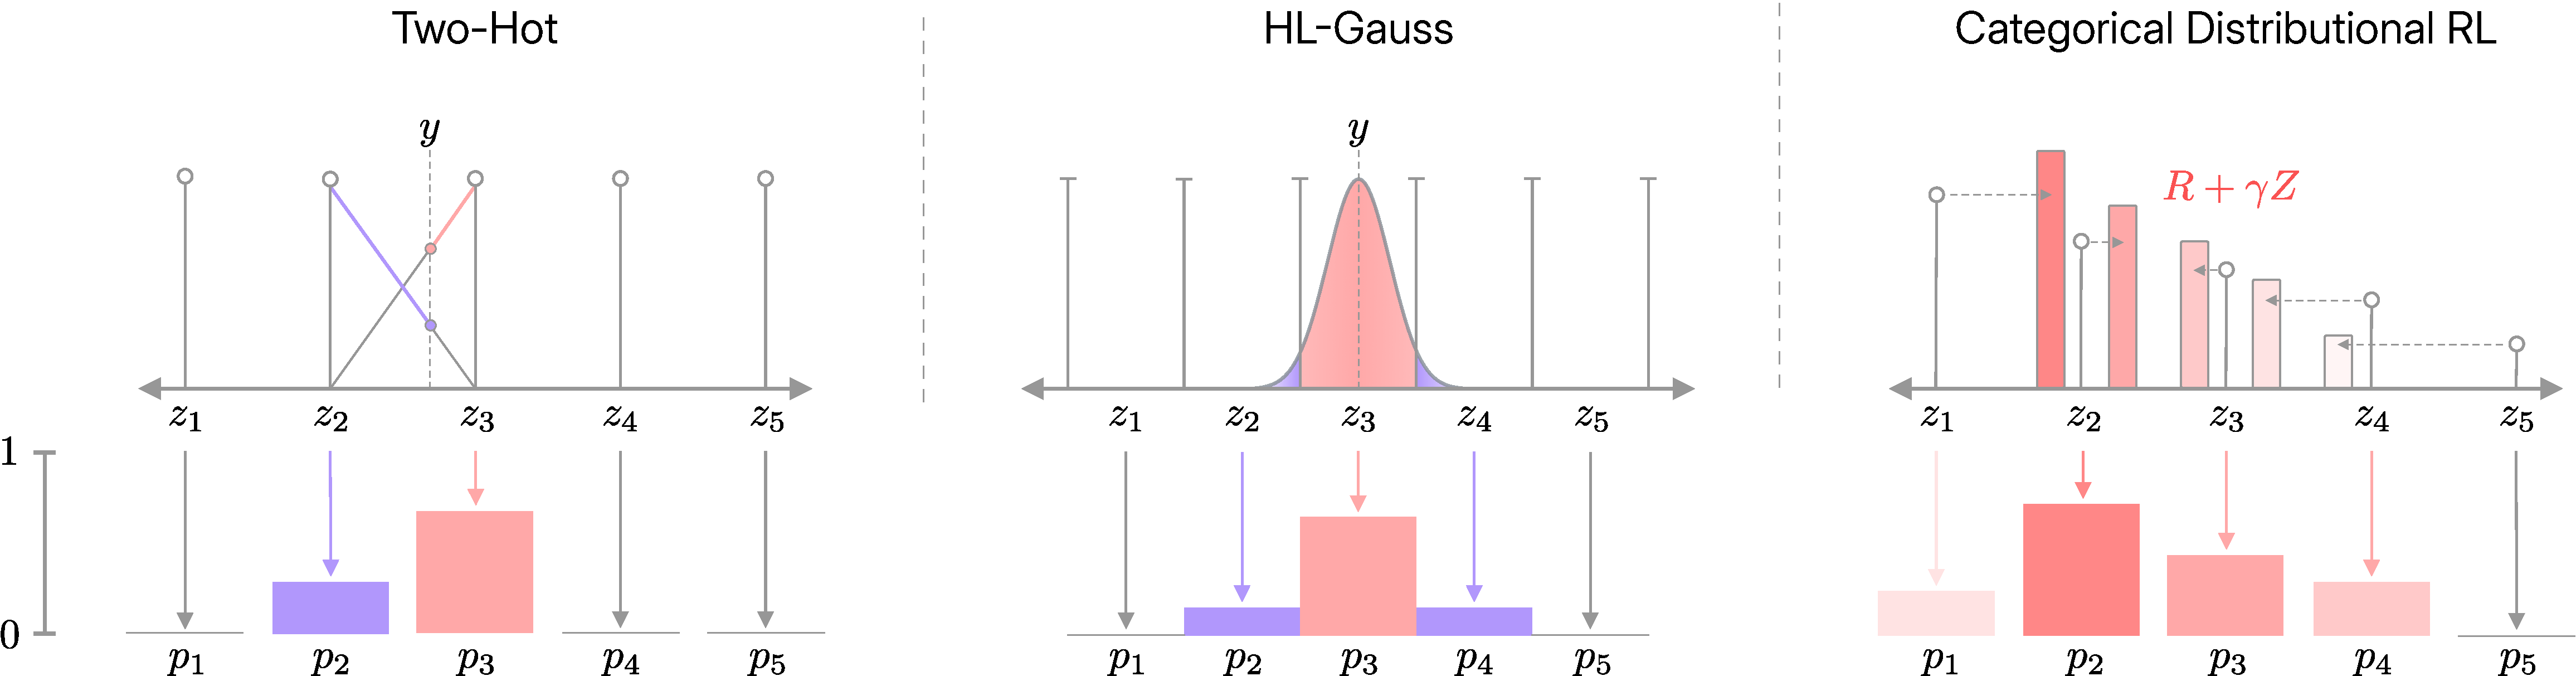
\includegraphics[height=1.5in]{figs/twoHot.pdf}
\caption{
  Illustration of how to encode a scalar target $y$
  or distributional target $Z$
using a categorical distribution.
\figtaken{Figure 1 of \citep{Farebrother2024}}.
\figthanks{Jesse Farebrother}.
}
\label{fig:twoHot}
\end{figure}


An alternative to quantile regression
is to approximate the distribution over returns
using a histogram, and then fit it
using cross entropy loss (see \cref{fig:twoHot}).
This approach was first suggested in \citep{Bellemare2017},
who called it  \keywordDef{categorical DQN}.
(In their paper, they use 51 discrete categories (atoms),
giving rise to the name \keywordDef{C51}.) 

An even simpler approach is to replace the distributional
target with the standard scalar target (representing the mean),
and then discretize this target
and use cross entropy loss instead of squared error.\footnote{
%
Technically speaking, this is no longer a distributional RL method,
since the prediction target is the mean,
but the mechanism for predicting the mean leverages a distribution,
for robustness and ease of optimization.
}
Unfortunately, this encoding is lossy.
In  \citep{Schrittwieser2020}, they
proposed the \keywordDef{two-hot} transform,
that is a lossless encoding of the target based on putting
appropriate weight on the nearest two bins (see \cref{fig:twoHot}).
In \citep{Imani2018}, they proposed the
\keywordDef{HL-Gauss} histogram loss,
that convolves the target value $y$ with a Gaussian,
and then discretizes the resulting continuous distribution.
This is  more symetric than two-hot encoding, as shown in \cref{fig:twoHot}.
Regardless of how the discrete target is chosen,
predictions are made using
$\hat{y}(s;\vtheta) = \sum_k p_k(s) b_k$,
where $p_k(s)$ is the probability of bin $k$,
and $b_k$ is the bin center.

In \citep{Farebrother2024}, they show that 
the HL-Gauss trick  works much better than
MSE,  two-hot and C51 across a variety of problems
(both offline and online),
especially  when they scale to large networks.
They conjecture that the reason it beats MSE
is that cross entropy is more robust to noisy targets
(e.g., due to stochasticity) and nonstationary targets.
They also conjecture  that the reason HL works better than two-hot
is that HL is closer to ordinal regression, and reduces overfitting
by having a softer (more entropic) target distribution
(similiar to label smoothing in classification problems).



\section{Reward functions}
\label{sec:reward}

Sequential decision making relies on the
 user to define the reward function in order to
 encourage the agent to exhibit some desired behavior.
In this section, we discuss this crucial aspect of the problem.
%However, sometimes we want or need to learn the reward function,
%as we discuss below.


\subsection{Reward hacking}
\label{sec:rewardHacking}
\label{sec:hacking}

In some cases, the reward function may be misspecified, so even though the agent may
maximize the reward, this might turn out not to be what the user desired.
For example, suppose the user rewards the agent for making as many
paper clips as possible.
An optimal agent may convert the whole world into a paper clip factory,
because the user forgot to specify various constraints, such as not
killing people or not destroying the environment.
In the \keywordDef{AI alignment} community,
this example is known as  the \keywordDef{paperclip maximizer problem},
and is due to Nick Bostrom \citep{Bostrom2016}.
(See e.g., \url{https://openai.com/index/faulty-reward-functions/} for some examples
that have occurred in practice.)
This is an example of a more general problem
known as
%\keywordDef{Goodhart's law} or
\keywordDef{reward hacking}
\citep{Skalse2022}.
For a potential solution, based on the assistance game paradigm,
see \cref{sec:assistance}.


\eat{
For example, a rat which can electrically stimulate its dopamine
center by pressing a lever, will press the lever indefinitely,
until it starves to death \citep{Bennett2023}; this is known as
\keywordDef{wire heading}, and illustrates
the dangers of changing the reward function.
}

\subsection{Sparse reward}

Even if the reward function is correct, optimizing it is not always easy.
In particular, many problems suffer from \keywordDef{sparse reward},
in which $R(s,a)=0$ for almost all states and actions, so the agent
only every gets feedback (either positive or negative) on the rare occasions
when it achieves some unknown goal.
This requires \keywordDef{deep exploration}
\citep{Osband2019}
to find the rewarding states.
One approach to this is use to use PSRL (\cref{sec:PSRL}).
However, various other heuristics have been developed,
some of which we discuss below.


\subsection{Reward shaping}
\label{sec:rewardShaping}

In  \keywordDef{reward shaping},
we add prior knowledge about what we believe good states should look like,
as a way to combat the difficulties of learning from sparse reward.
That is, we define a new reward function $r' = r + F$,
where $F$ is called the shaping function.
In general, this can affect the optimal policy.
For example, if a soccer playing agent is ``artificially''
rewarded for making contact with the ball,
it might learn to repeatedly touch and untouch the ball
(toggling between $s$ and $s'$), rather than
trying to win the original game.
But in \citep{Ng99},
the prove that if the shaping function has the form
\be
F(s,a,s') = \gamma \Phi(s') - \Phi(s)
\ee
where $\Phi: \calS \ra \real$
is a \keywordDef{potential function},
then we can guarantee that the sum of shaped rewards
will match the sum of original rewards plus a constant.
This is called \keywordDef{Potential-Based Reward Shaping}.

In \citep{Wiewiora2003}, they prove that (in the tabular case)
this approach
is equivalent to initializing the value function
to $V(s)=\Phi(s)$.
%In \citep{Wiewiora2003aaai}, 
In \citep{Tessler2019},
they propose
an extension called potential-based advice,
where they show that a potential of the form
$F(s,a,s',a') = \gamma \Phi(s',a') - \Phi(s,a)$
is also valid (and more expressive).
In \citep{Hu2020}, they introduce a reward shaping function $z$
which can be used to down-weight or up-weight the
shaping function:
\be
r'(s,a) = r(s,a) + z_{\phi}(s,a) F(s,a)
\ee
They use bilevel optimization to optimize $\phi$
wrt the original task performance.


% https://gibberblot.github.io/rl-notes/single-agent/reward-shaping.html#potential-based-reward-shaping
%



\subsection{Intrinsic reward}
\label{sec:intrinsicReward}
\label{sec:intrinsic}

When the extrinsic reward is sparse,
it can be useful to (also) reward the agent for solving
``generally useful'' tasks,
such as learning about the world.
This is called \keywordDef{intrinsically motivated RL}
\citep{Aubret2023,Linke2019,Amin2021,Yuan2022,Yuan2024,Colas2022}.
It can be thought of as a special case of reward shaping,
where the shaping function is dynamically computed.

We can classify these methods into two main types:
\keywordDef{knowledge-based intrinsic motivation},
or \keywordDef{artificial curiosity},
where the agent is
rewarded for learning about its environment;
and  \keywordDef{competence-based intrinsic motivation},
where the agent is rewarded for achieving novel goals
or mastering new skills.

\subsubsection{Knowledge-based intrinsic motivation}

One simple approach to knowledge-based intrinsic motivation
is to add to the extrinsic reward
an intrinsic \keywordDef{exploration bonus}
$R_t^i(s_t)$,
which is high when the agent visits novel states.
For tabular environments, we can just count the number of visits to each state,
$N_t(s)$, and define $R_t^i(s) = 1/N_t(s)$ or
$R_t^i(s) = 1/\sqrt{N_t(s)}$, which is similar to the UCB
heuristic used in bandits (see \cref{sec:UCB}).
We can  extend exploration bonuses  to high dimensional states (e.g. images)
using density models \citep{Bellemare2016}.
Alternatively, \citep{Machado2020} propose to use the $\ell_1$
norm of the successor feature (\cref{sec:SF}) representation
as an alternative to the visitation count, giving rise
to an intrinsic reward of the form
$R^i(s) = 1/||\vpsi^{\pi}(s)||_1$.
Recently \citep{Yu2023} extended this to combine
SFs with {\em predecessor} representations,
which encode retrospective information about the previous state
(c.f., inverse dynamics models, mentioned below).
This encourages exploration towards bottleneck states.

Another approach
is the \keywordDef{Random Network Distillation} or \keywordDef{RND}
method of \citep{Burda2018}.
This uses a fixed random neural network feature extractor
$\vz_t=f(\vs_t;\vtheta^*)$ to define a target,
and then trains a predictor $\hat{\vz}_t=f(\vs_t;\hat{\vtheta}_t)$
to predict these targets.
If $\vs_t$ is similar to previously seen states,
then the trained model will have low prediction error.
We can thus define the intrinsic reward as proportional
to the squared error $||\hat{\vz}_t - \vz_t||_2^2$.
%In  \citep{Burda2018}, they show that this metric
%is related to the predictive uncertainty
%of a deep ensemble with a random prior
%\cref{sec:rndPrior}.
The \keywordDef{BYOL-Explore} method of
\citep{Guo2022} goes beyond RND by learning
the target representation (for the next state),
rather than using a fixed random projection,
but is still based on prediction error.


\eat{
The value function now has two output heads,
one to predict the sum of extrinsic rewards,
and another to predict the sum of intrinsic rewards;
the latter can change over time as the agent learns.
The overall value is the sum of these two heads,
similar to the reward shaping term
$V(s;\vw) = V^e(s;\vw) + V^i(s;\vw')$ in \cref{sec:rewardShaping}.

The RND method has given good results on Atari games
with sparse reward, such as \keyword{Montezuma's revenge}.
as well as some continuous control problems
\citep{Laskin2021}.
}

We can also define an intrinsic reward in terms
of the information theoretic \keywordDef{surprise}
of the next state given the current one:
\be
R(\vs,\va,\vs') = -\log q(\vs'|\vs,\va)
\ee
This is the same as methods based on
rewarding states for prediction error.
Unfortunately such methods
can suffer from 
the \keywordDef{noisy TV problem}
(also called a \keywordDef{stochastic trap}),
in which an agent is attracted to states 
which are intrinsically to predict.
To see this, note that by averaging
over future states we see that the above reward reduces to
\be
R(\vs,\va) = -\expectQ{\log q(\vs'|\vs,\va)}{p^*(\vs'|\vs,\va)}
= \crossentropy(p^*, q)
\ee
where $p^*$ is the true model and $q$ is the learned dynamics model,
and $\crossentropy$ is the cros -entropy.
As we learn the optimal model, $q=p^*$,
this reduces to the conditional
entropy of the predictive distribution,
which can be non-zero for inherently unpredictable states.

To help filter out such random noise,
\citep{Pathak2017} proposes an
\keywordDef{Intrinsic Curiosity Module}.
This first learns  an \keywordDef{inverse dynamics model}
of the form $a = f(\vs,\vs')$, which tries
to predict which action was used, given
that the agent was in $\vs$ and is now in $\vs'$.
The classifier has the form
$\softmax(g(\phi(\vs), \phi(s'), a))$,
where $\vz=\phi(\vs)$ is  a representation function
that focuses  on parts of the state that the agent can control.
Then the agent learns a forwards dynamics model
in $\vz$-space.
Finally it defines the intrinsic reward as
\be
R(\vs,\va,\vs') = -\log q(\phi(\vs')|\phi(\vs),a)
\ee
Thus the agent is rewarded for visiting states that lead
to unpredictable consequences,
where the difference in outcomes is measured
in a (hopefully more meaningful) latent space.

Another solution  is to replace the cross entropy
with the KL divergence,
$R(\vs,\va) = \KL(p||q) = \crossentropy(p,q) - \entropy(p)$,
which goes to zero once the learned model matches the true model,
even for unpredictable states.
This has the desired effect of encouraging exploration towards states
which have epistemic uncertainty (reducible noise)
but not aleatoric uncertainty (irreducible noise)
\citep{Mavor-Parker2022}.
The \keywordDef{BYOL-Hindsight} method of \citep{Jarrett2023}
is one recent approach that attempts to use
the $R(\vs,\va) = \KL(p||q)$ objective.
Unfortunately, computing the $\KL(p||q)$ term is much harder
than the usual variational objective of $\KL(q||p)$.
A related idea,
proposed in the RL context by \citep{Schmidhuber2010},
is to use the \keywordDef{information gain} as a reward.
This is defined as
$R_t(\vs_t,\va_t)=\KL(q(\vs_t|\vh_t,\va_t,\vtheta_t)
|| q(\vs_t|\vh_t,\va_t,\vtheta_{t-1})$,
where $\vh_t$ is the history of past observations,
and $\vtheta_t=\text{update}(\vtheta_{t-1}, \vh_t, \va_t, \vs_t)$
are the new model parameters.
This is closely related to the BALD (Bayesian Active Learning by Disagreement)
criterion
\citep{Houlsby2011,Kirsch2019},  and has the advantage
of being  easier to compute, since it is does not reference
the true distribution $p$.
%https://people.idsia.ch/~juergen/artificial-curiosity-since-1990.html
%https://ae-foster.github.io/posts/2022/04/27/bed-bald.html



%See also e.g., \citep{Amin2021,Yuan2022} for a recent survey other intrinsic reward methods.

\subsubsection{Goal-based intrinsic motivation}
%\subsection{Go Explore: TODO}
\label{sec:goExplore}



We will discuss goal-conditioned RL
in \cref{sec:GCRL}. If the agent creates its own goals,
then it provides a way to explore the environment.
The question of when and how an agent to switch to pursuing
a new goal is studied in \citep{Pislar2022}
(see also \citep{Bagaria2023}).
Some other key work in this space includes
the \keywordDef{scheduled auxiliary control}
method of \citep{Riedmiller2018},
and
the \keywordDef{Go Explore} algorithm in 
\citep{Ecoffet2019,Ecoffet2021}
and its recent LLM extension \citep{Lu2024go}.



\eat{
\subsection{Meta-learning the reward function}
\label{sec:rewardMeta}

It may be possible to learn the reward function
using  \keywordDef{bilevel optimization problem},
where the outerloop searches over reward functions,
and the inner loop searches over policies that maximize the given reward.
The value returned by the inner loop is the score which is maximized by the outer loop.
This is analogous to evolution, which searches 
over reward functions, such as the desire for food and sex,
which are then optimized by the agent using RL.
Evolution's goal is to maximize the evolutionary fitness of each agent,
which cannot be directly measured by the agent itself,
but can be estimated at a population level.
See also \cref{sec:LLMreward}.
}



\section{Hierarchical RL}
\label{sec:HRL}

%https://thegradient.pub/the-promise-of-hierarchical-reinforcement-learning/
%https://x.com/RichardSSutton/status/1813987506200957103
%https://github.com/Jinjiarui/hrl-papers

So far we have focused on MDPs that work at a single time scale.
However, this is very limiting.
For example, imagine planning a trip from San Francisco to New York:
we need to choose high level actions first, such as which airline to fly,
and then medium level actions, such as how to get to the airport,
followed by low level actions, such as motor commands.
Thus we need to consider actions that operate multiple levels
of \keywordDef{temporal abstraction}.
This is called \keywordDef{hierarchical RL} or \keywordDef{HRL}.
This is a big and important topic,
and we only brief mention a few key ideas and methods.
Our summary is based in part on 
\citep{Pateria2022}.
(See also \cref{sec:beyond} where we discuss multi-step
predictive models; by contrast, in this section we focus
on model-free methods.)
% Hutsebaut-Buysse2022,

\subsection{Feudal (goal-conditioned) HRL}
\label{sec:feudal}
\label{sec:GCRL}

\begin{figure}
\centering
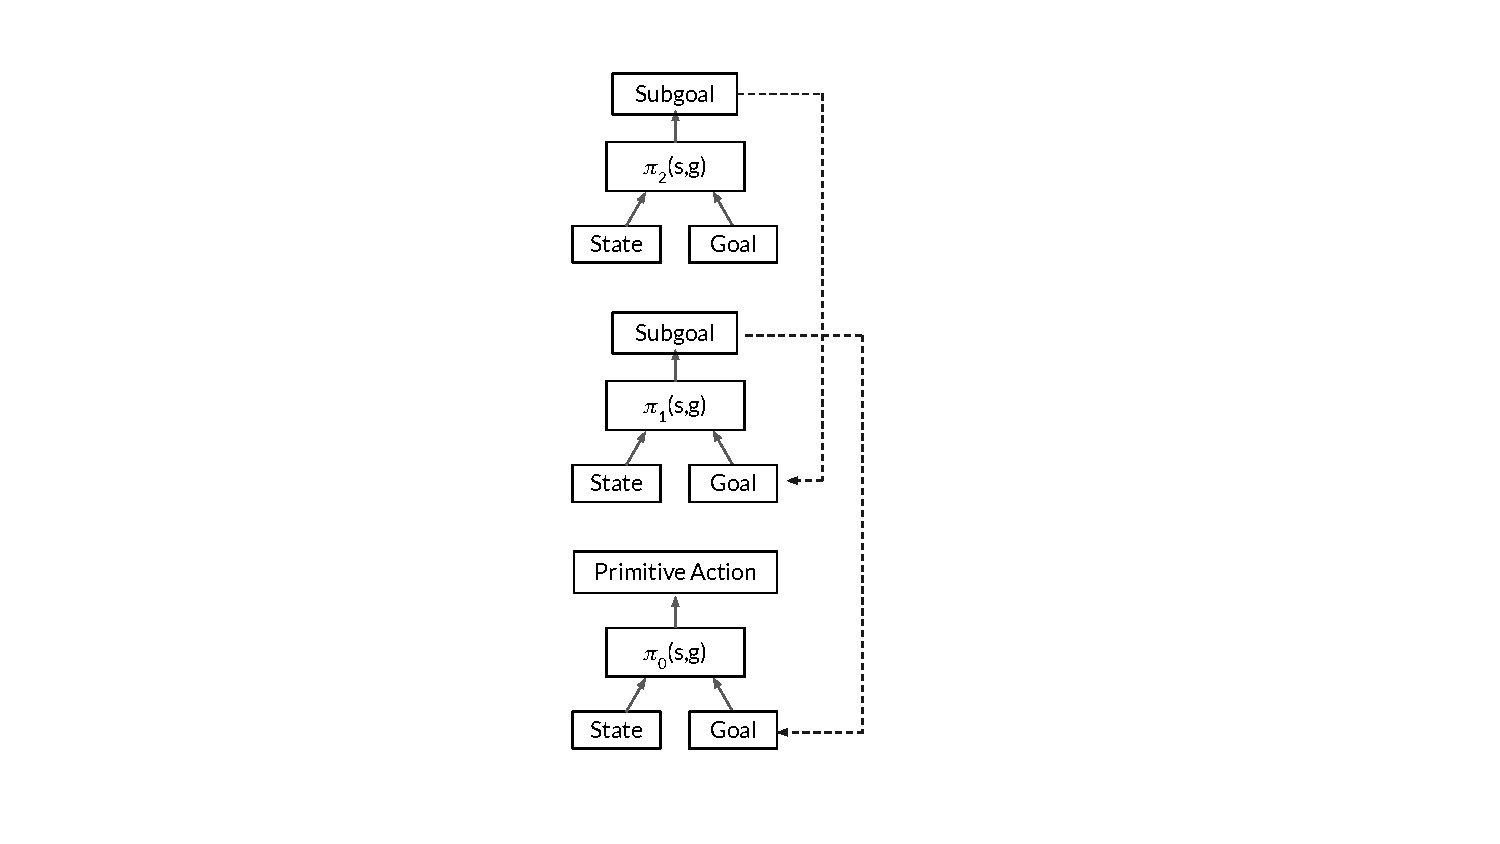
\includegraphics[height=2.5in]{figs/Goal_Cond_HRL_Architecture.pdf}
\caption{
  Illustration of a 3 level hierarchical goal-conditioned controller.
\figtaken{\url{http://bigai.cs.brown.edu/2019/09/03/hac.html}}.
\figthanks{Andrew Levy}.
}
\label{fig:HAC}
\end{figure}

In this section, we discuss an approach to HRL known as
\keywordDef{feudal RL} \citep{Dayan1992}. Here the action
space of the higher level policy consists of \keywordDef{subgoals}
that are passed down to the lower level policy.
See \cref{fig:HAC} for an illustration.
The lower level policy learns a \keywordDef{universal policy}
$\pi(a|s,g)$, where $g$ is the goal passed into it
\citep{Schaul2015}.
This policy
optimizes an MDP in which the reward is define as $R(s,a|g)=1$
iff the goal state is achieved,
i.e., $R(s,a|s) = \ind{s=g}$.
(We can also define a dense reward signal using
some state abstraction function $\phi$,
by definining $R(s,a|g)=\text{sim}(\phi(s), \phi(g))$
for some similarity metric.)
This approach to RL is known as
\keywordDef{goal-conditioned RL} \citep{Liu2022GCL}.
%The set of goals can be manually defined or discovered,
%as we discuss below.


\subsubsection{Hindsight Experience Relabeling (HER)}
\label{sec:HER}


In this section, we discuss an approach to efficiently learning
goal-conditioned  policies,
in the special case where
the set of goal states
$\calG$ is the same as the set of original states $\calS$.
We will extend this to the hierarchical case below.

The basic idea is as follows.
We collect various trajectores  in the environment,
from a starting state $s_0$ to some terminal state $s_T$,
and then define the goal of each trajectory as being $g=s_T$;
this trajectory then serves as a demonstration
of how to achieve this goal.
This is called \keywordDef{hindsight experience relabeling}
or \keywordDef{HER} \citep{HER}.
This can be used to relabel the trajectories stored in the replay buffer.
That is, if we have $(s,a,R(s|g),s',g)$ tuples, we replace them with
$(s,a,R(s|g'),g')$ where $g'=s_T$.
We can then use any off-policy RL method to learn $\pi(a|s,g)$.
In \citep{Eysenbach2020}, they show that HER can be viewed as a special
case of maximum-entropy inverse RL,
since it is estimating the reward for which the corresponding
trajectory was optimal.

\subsubsection{Hierarchical HER}
\label{sec:HAC}
\label{sec:HIRO}

We can leverage HER to learn a hierarchical controller
in several ways. In \citep{Nachum2018}
they propose \keywordDef{HIRO}
(Hierarchical Reinforcement Learning with Off-policy Correction)
as a way to train a two-level controller.
(For a two-level controller, the top level is often
called the \keywordDef{manager}, and the low level the \keywordDef{worker}.)
The data for the manager are transition tuples
of the form $(s_t, g_t, \sum r_{t:t+c}, s_{t+c})$,
where $c$ is the time taken for the worker to
reach the goal (or some maximum time),
and $r_t$ is the main task reward function at step $t$.
The data for the worker are transition tuples of the form
$(s_{t+i}, g_t, a_{t+i}, r_{t+i}^{g_t}, s_{t+i+1})$
for $i=0:c$, where $r_t^{g}$ is the reward
wrt reaching goal $g$.
This data can be used to train the two policies.
However, if the worker fails to achieve the goal
in the given time limit,
all the rewards will be 0, and no learning will take place.
To combat this,
if the worker does not achieve $g_t$
after $c$ timesteps, the subgoal is relabeled
in the transition data with another subgoal $g_t'$
which is sampled from $p(g|\tau)$,
where $\tau$ is the observed trajectory.
Thus both policies treat $g_t'$ as the goal in hindsight,
so they can use the actually collected data for training


%Unfortunately, training all levels of the hierarchy at the same time
%can be unstable.
The \keywordDef{hierarchical actor critic} (HAC) method
of \citep{Levy2018} is a simpler version of HIRO that can be extended
to multiple levels of hierarchy,
where the lowest level corresponds to primitive actions
(see \cref{fig:HAC}).
In the HAC approach, the output subgoal in the higher level data,
and the input subgoal in the lower-level data,
are replaced with the actual state that was achieved
in hindsight. This allows
the training of  each level of the
hierarchy independently of the lower levels,
by assuming  the lower level policies are already optimal
(since they achieved the specified goal).
As a result, the distribution of
$(s,a,s')$ tuples experienced by a higher level
will be stable,  providing a  stationary learning target.
By contrast, if all policies are learned simultaneously,
the distribution becomes \keywordDef{non-stationary},
which makes learning harder.
For more details, see the paper,
or the corresponding blog post (with animations)
at  \url{http://bigai.cs.brown.edu/2019/09/03/hac.html}.
%(Note that \citep{McClinton2021} combines HAC
%with intrinsic reward (\cref{sec:intrinsic})
%to improve exploration.)


\subsubsection{Learning the subgoal space}

In the previous approaches, the subgoals are defined
in terms of the states that were achieved at the end
of each trajectory, $g'=s_T$. This can be generalized
by using a state abstraction function to get
$g'=\phi(s_T)$.
The methods in \cref{sec:HIRO})
assumed that $\phi$ was manually
specified.
We now mention some ways to learn $\phi$.

In \citep{Vezhnevets2017}, they present
\keywordDef{Feudal Networks} for learning a two level hierarchy.
The manager samples subgoals in a learned latent subgoal space.
The worker uses distance to this subgoal as a reward,
and is trained in the usual way.
The manager uses the ``transition gradient'' as a reward,
which is derived from the task reward as well as the
distance between the subgoal and the actual state transition
made by the worker. This reward signal is used to learn
the manager policy and the latent subgoal space.

Feudal networks do not guarantee that the learned subgoal
space will result in optimal behavior.
In \citep{Nachum2019}, they present
a method to optimize the policy and $\phi$ function
so as to minimize a bound on the suboptimality of the hierarchical
policy.
This approach is combined with HIRO
(\cref{sec:HIRO}) to tackle the non-stationarity issue.



\subsection{Options}
\label{sec:options}

The feudal approach to HRL is somewhat limited,
since not all subroutines or skills can be defined in terms
of reaching a goal state (even if it is a partially
specified one, such as being in a desired location
but without specifying the velocity).
For example, consider the skill of
``driving in a circle'', or ``finding food''.
The \keywordDef{options} framework  is a
more general framework for HRL first proposed in
\citep{options}.
We discuss this below.

\subsubsection{Definitions}

An option $\omega=(I,\pi,\beta)$ is a tuple consisting of:
the \keywordDef{initiation set} $I_{\omega} \subset S$,
which is a subset of states that this option can start from
(also called the \keywordDef{affordances} of  each state
\citep{Khetarpal2020});
the \keywordDef{subpolicy} $\pi_{\omega}(a|s) \in [0,1]$;
and the \keywordDef{termination condition}
$\beta_{\omega}(s) \in [0,1]$,
which gives the probability of finishing in state $s$.
(This induces a geometric distribution over option durations,
which we denote by $\tau \sim \beta_{\omega}$.)
The set of all options is denoted $\Omega$.

To execute an option at step $t$ entails choosing an action using
$a_t = \pi_{\omega}(s_t)$ and then deciding whether
to terminate at step $t+1$ with probability
$1-\beta_{\omega}(s_{t+1})$ or to continue following the option at step $t+1$.
(This is an example of a \keywordDef{semi-Markov decision process}
\citep{Puterman94}.)
If we define $\pi_{\omega}(s)=a$ and $\beta_{\omega}(s)=0$ for all $s$, then
this option corresponds to primitive action $a$ that terminates in one step.
But with options we can expand the repertoire of actions to include those that
take many steps to finish.

To create an MDP with options, we need to define the reward function
and dynamics model. The reward is defined as follows:
\be
R(s,\omega) = \expect{R_1 + \gamma R^2 + \cdots + \gamma^{\tau-1} R_{\tau}
  \vert S_0=s, A_{0:\tau-1} \sim \pi_{\omega}, \tau \sim \beta_{\omega} }
\ee
The dynamics model is defined as follows:
\be
p_{\gamma}(s'|s,\omega) = \sum_{k=1}^{\infty}
\gamma^k \Pr\left(S_k=s', \tau=k | S_0=s, A_{0:k-1} \sim \pi_{\omega},
\tau \sim \beta_{\omega}\right)
\ee
Note that $p_{\gamma}(s'|s,\omega)$ is not a conditional probability distribution,
because of the $\gamma^k$ term,
but we can usually treat it like one.
Note also that a dynamics model  that can predict multiple steps ahead
is sometimes called a \keywordDef{jumpy model}
(see also \cref{sec:jumpy}).



We can use these
definitions to define the value function for a hierarchical policy
using a generalized Bellman equation, as follows:
\be
V_{\pi}(s) = \sum_{\omega  \in \Omega(s)}
\pi(\omega|s)
\left[ R(s,\omega) + \sum_{s'} p_{\gamma}(s'|s,\omega)  V_{\pi}(s') \right]
\ee
We can compute this using value iteration.
We can  then learn a policy using
policy iteration, or a policy gradient method.
In other words, once we have defined the options,
we can use all the standard RL machinery.

Note that GCRL can be considered a special case of options
where each option corresponds to a different goal.
Thus the reward function has the form
$R(s,\omega)=\ind{s=\omega}$,
the termination function is
$\beta_{\omega}(s)=\ind{s=\omega}$,
and
the initiation set is the entire state space.

\subsubsection{Learning options}

The early work on options,
including the \keywordDef{MAXQ} approach of
\citep{Dietterich2000hrl},
assumed that the set of options was manually specified.
Since then, many methods for learning options have been proposed.
We mention a few of these below.


The first set of methods for option learning
rely on two stage training.
In the first stage, exploration methods
are used to collect trajectories.
Then this data is analysed, 
either by inferring hidden segments
using EM applied to a latent variable model
\citep{Daniel2016},
or  by using
the \keywordDef{skill chaining} method
of \citep{Konidaris2009},
which uses
classifiers to segment the trajectories.
The labeled data can then be used to define
a set of options, which can be trained using standard methods.



The second set of methods for option learning
use end-to-end training,
i.e., the options and their policies are jointly learned online.
For example,
\citep{Bacon2017} propose the  \keywordDef{option-critic} architecture.
The number of options is manually specified,
and all policies are randomly initialized.
Then they are jointly trained using policy gradient methods
designed for semi-MDPs.
(See also \citep{Riemer2018} for a hierarchical
extension of option-critic to support options calling options.)
%This has been extended in various ways,
%e.g., with attention \citep{Chunduru2020}
However, since the learning signal is just the main task reward,
the method can work poorly
in problems with sparse reward compared to
subgoal methods
(see discussion in \citep{Vezhnevets2017,Nachum2019}).

Another problem with option-critic is that it requires
specialized methods that are designed for optimizing semi-MDPs.
In \citep{Zhang2019dac}, they propose
\keywordDef{double actor critic},
which allows the use of standard policy gradient methods.
This works  by defining two parallel
\keywordDef{augmented MDPs},
where the state space of each MDP is the cross-product
of the original state space and the set of options.
The manager learns a policy over options,
and the worker learns a policy over states for each option.
Both MDPs just use task rewards, without subgoals or
subtask rewards.

It has been observed that
option learning using option-critic or double actor-critic can fail,
in the sense that the top level controller
may learn to switch from one option to the next at almost
every time step
\citep{Zhang2019dac,Harb2018}.
The reason is that the
optimal policy does not require
the use of temporally extended options,
but instead can be defined in terms of primitive actions
(as in standard RL).
Therefore in
\citep{Harb2018} they propose to add a regularizer
called the \keywordDef{deliberation cost},
in which the higher level policy is penalized
whenever it switches options.
This can speed up learning, at the cost of a potentially
suboptimal policy.

Another possible failure mode in option learning
is if the higher level policy selects a single
option for the entire task duration.
To combat this, \citep{Khetarpal2019} propose the
\keywordDef{Interest Option Critic},
which learns the  initiation condition $I_{\omega}$
so that the option is selected
only in certain states of interest,
rather than the entire state space.

In \citep{Machado2023}, they discuss how the successor
representation (discussed in \cref{sec:successor})
can be used to define options,
using a method they call the \keywordDef{Representation-driven
  Option Discovery} (ROD) cycle.
% https://medium.com/@marlos.cholodovskis/the-representation-driven-option-discovery-cycle-e3f5877696c2

In \citep{Lin2024nips} they propose to represent options as programs,
which are learned using LLMs.

\eat{
Unfortunately,  it is currently unclear how best
to learn options  automatically,
although there has been some work
(see e.g.,  \citep{Ramesh2019,Sutton2023}).
See also \cref{sec:HER} where we discuss an alternative approach to
HRL using goal-conditioned policies.

So far, we have assumed the set of goals is pre-specified
(or can be derived using HER with a fixed function $\phi$).
There have been several proposals on how to automatically
learn good goals.
\citep{Choi2021} propose a variational approach to
\keywordDef{empowerment}, that
tries to maximize the mutual information between the agent’s actions or goals
and its experienced states.
}



%\section{Distributional RL}
%\label{sec:distributional}

%We work with distributions of rewards
%instead of  expected rewards \citep{Bellemare2017,BellemareBook}.




\section{Imitation learning}
\label{sec:imitation}

In previous sections, an RL agent is
to learn an optimal sequential decision making policy
so that the total reward is maximized.
\keywordDef{Imitation learning} (IL),
also known as \keywordDef{apprenticeship learning}
and \keywordDef{learning from demonstration} (LfD),
is a different setting,
in which the agent does not observe rewards,
but has access to a collection $\dataExp$ of trajectories
generated by an expert policy $\policyexp$;
that is, $\traj = (s_0,a_0,s_1,a_1,\ldots,s_T)$
and $a_t \sim \policyexp(s_t)$
for $\traj\in\dataExp$.
The goal is to learn a good policy by imitating the expert,
in the absence of reward signals.
IL finds many applications in scenarios
where we have demonstrations of experts (often humans)
but designing a good reward function is not easy,
such as car driving and conversational systems.
(See also \cref{sec:offlineRL}, where we discuss the closely
related topic of offline RL, where we also learn from a collection
of trajectories, but no longer assume they are generated by an optimal
policy.)

\subsection{Imitation learning by behavior cloning}
\label{sec:behavior-cloning}
\label{sec:BC}

A natural method is \keywordDef{behavior cloning},
which reduces IL to supervised learning;
see \citep{Pomerleau89} for an early application
to autonomous driving.
It interprets a policy as a classifier that
maps states (inputs) to actions (labels),
and finds a policy
by minimizing the imitation error, such as
\begin{align}
\label{eqn:rl-inference-bc}
\min_{\policy}
\expectQ{\KLpq{\policyexp(s)}{\policy(s)}}{\statdistpolexp(s)}
\end{align}
where the expectation wrt $\statdistpolexp$ may be approximated by averaging over states in $\dataExp$.
A challenge with this method is that the loss
does not consider the sequential nature of IL:
future state distribution is not fixed
but instead depends on earlier actions.
Therefore, if we learn a policy $\hat{\policy}$ that
has a low imitation error under distribution
$\statdistpolexp$,
as defined in \cref{eqn:rl-inference-bc},
it may still incur a large error
under distribution $\statdist_{\hat{\policy}}$
(when the policy $\hat{\policy}$ is actually run).
This problem has been tackled by the offline RL
literature, which we discuss in \cref{sec:offlineRL}.

\eat{
Further expert demonstrations
or algorithmic augmentations are often
needed to handle the distribution mismatch
(see e.g., \citep{Daume09,Ross11}).
}

\subsection{Imitation learning by inverse reinforcement learning}
\label{sec:IRL}

An effective approach to IL is 
\keywordDef{inverse reinforcement learning} (IRL)
or \keywordDef{inverse optimal control} (IOC).
Here, we first infer a reward function
that ``explains'' the observed expert trajectories,
and then compute a (near-)optimal policy
against this learned reward using any standard
RL algorithms studied in earlier sections.
The key step of reward learning 
(from expert trajectories)
is the opposite of standard RL,
thus called inverse RL~\citep{Ng00irl}.

It is clear that there are infinitely many reward functions for which the expert policy is optimal,
for example by several optimality-preserving transformations~\citep{Ng99}.
To address this challenge,
we can follow the maximum entropy principle,
and use an energy-based probability model
to capture how expert trajectories are
generated~\citep{Ziebart08}:
\begin{align}
p(\traj) \propto 
%\exp(R_{\vtheta}(\traj)) = 
\exp\big(\sum_{t=0}^{T-1} R_{\vtheta}(s_t,a_t)\big)
\end{align}
where $R_{\vtheta}$ is an 
unknown reward function with parameter $\vtheta$.
Abusing notation slightly, we denote by
$R_{\vtheta}(\traj) = \sum_{t=0}^{T-1} R_{\vtheta}(s_t,a_t))$
the cumulative reward along the trajectory $\traj$.
This model assigns exponentially small probabilities
to trajectories with lower cumulative rewards.
The partition function,
$Z_{\vtheta} \defeq \int_{\traj}\exp(R_{\vtheta}(\traj))$,
is in general intractable to compute,
and must be approximated.
Here, we can take a sample-based approach.
Let $\dataExp$ and $\data$ be the sets of
trajectories generated by an expert,
and by some known distribution $q$, respectively.
We may infer $\vtheta$ by maximizing the likelihood,
$p(\dataExp|\vtheta)$,
or equivalently,
minimizing the negative log-likelihood loss
\begin{align}
\loss(\vtheta) &= -\frac{1}{|\dataExp|}\sum_{\traj\in\dataExp} R_{\vtheta}(\traj) + \log \frac{1}{|\data|}\sum_{\traj\in\data} \frac{\exp(R_{\vtheta}(\traj))}{q(\traj)}
\end{align}
The term inside the $\log$ of the loss is an
importance sampling estimate of $Z$
that is unbiased as long as $q(\traj)>0$ for all $\traj$.
However, in order to reduce the variance,
we can choose $q$ adaptively
as $\vtheta$ is being updated.
The optimal sampling distribution,
$q_*(\traj) \propto \exp(R_{\vtheta}(\traj))$,
is hard to obtain.  Instead, we may find
a policy $\hat{\policy}$
which induces a distribution that is close to $q_*$,
for instance, using methods of maximum entropy RL discussed in \cref{sec:maxentRL}.
Interestingly, the process above produces
the inferred reward $R_{\vtheta}$
as well as an approximate optimal policy $\hat{\policy}$.
This approach is used by \keywordDef{guided cost learning}~\citep{Finn2018GCL},
and found effective in robotics applications.


\subsection{Imitation learning by divergence minimization}
\label{sec:ildm}

We now discuss a different, but related, approach to IL.
Recall that the reward function depends only on
the state and action in an MDP.
It implies that if we can find a policy $\policy$,
so that $\statdistpol(s,a)$ and $\statdistpolexp(s,a)$ are close,
then $\policy$ receives similar long-term reward
as $\policyexp$,
and is a good imitation of $\policyexp$ in this regard.
A number of IL algorithms find $\policy$
by minimizing the divergence between
$\statdistpol$ and $\statdistpolexp$.
We will largely follow the exposition of \citep{Ghasemipour19};
see \citep{Ke19} for a similar derivation.

Let $f$ be a convex function,
and $\fdiv$ be the corresponding $f$-divergence
\citep{Morimoto1963,Ali1966,Csiszar1967,liese2006divergences,csiszar2004information}.
From the above intuition, we want to minimize
$\fdivpq{\statdistpolexp}{\statdistpol}$.
Then, using a variational approximation of
$\fdiv$~\citep{Nguyen2010},
we can solve the following optimization problem for $\policy$:
\begin{align}
\label{eqn:rl-inference-ildm}
\min_{\policy} \max_{\vw}
\expectQ{T_{\vw}(s,a)}{\statdistpolexp(s,a)}
- \expectQ{f^*(T_{\vw}(s,a))}{\statdistpol(s,a)}
\end{align}
where $f^*$ is the convex conjugate of $f$,
and $T_{\vw}:\calS\times\calA\to\real$
is some function parameterized by $\vw$.
We can think of $\pi$ as a generator (of actions)
and $T_{\vw}$ as an adversarial critic
that is used to compare the generated $(s,a)$
pairs to the real ones.
Thus
the first expectation can be estimated using
$\dataExp$, as in behavior cloning,
and the second can be estimated using trajectories
generated by policy $\policy$.
Furthermore, to implement this algorithm, we often
use a parametric policy representation $\polapprox$,
and then perform stochastic gradient updates to
find a saddle-point to \cref{eqn:rl-inference-ildm}.
%
With different choices of the convex function $f$,
we can obtain many existing IL algorithms,
such as 
%behavior cloning (\cref{eqn:rl-inference-bc}),
%DAgger~\citep{Ross11},
\keywordDef{generative adversarial imitation learning}
(\keywordDef{GAIL})~\citep{Ho16}
and
\keywordDef{adversarial inverse RL}
(\keywordDef{AIRL})~\citep{Fu18},
etc.

\eat{
Finally, the algorithms above typically require
running the learned policy $\policy$ 
to approximate the second expectation
in \cref{eqn:rl-inference-ildm}.
In risk- or cost-sensitive scenarios,
collecting more data is not always possible,
Instead, we are in the off-policy IL setting,
working with trajectories collected by some policy
other than $\policy$.
Hence, we need to correct the mismatch
between $\statdistpol$ and
the off-policy trajectory distribution,
for which techniques from \cref{sec:offpolicyRL}
can be used.
An example is
\keywordDef{ValueDICE}~\citep{Kostrikov2020},
which uses a similar distribution correction
method of DualDICE~(\cref{sec:offpolicyrl-dice}).
}

\eat{
By the idea of matching (cite Abbeel-Ng)
f-MAX (4)
JS-div leads to GAIL
ReverseKL leads to AIRL
GAIL is more general?
Connection to DICE
\citep{Ghasemipour19,Abbeel04,Ho16}
\citep{Kostrikov2020}

Mention other imitation learning (apprenticeship learning, IOC) methods:
behavior cloning, by GD (Neu), by LP (Bowling)
}



\section{Offline RL}
\label{sec:offlineRL}

\begin{figure}
\centering
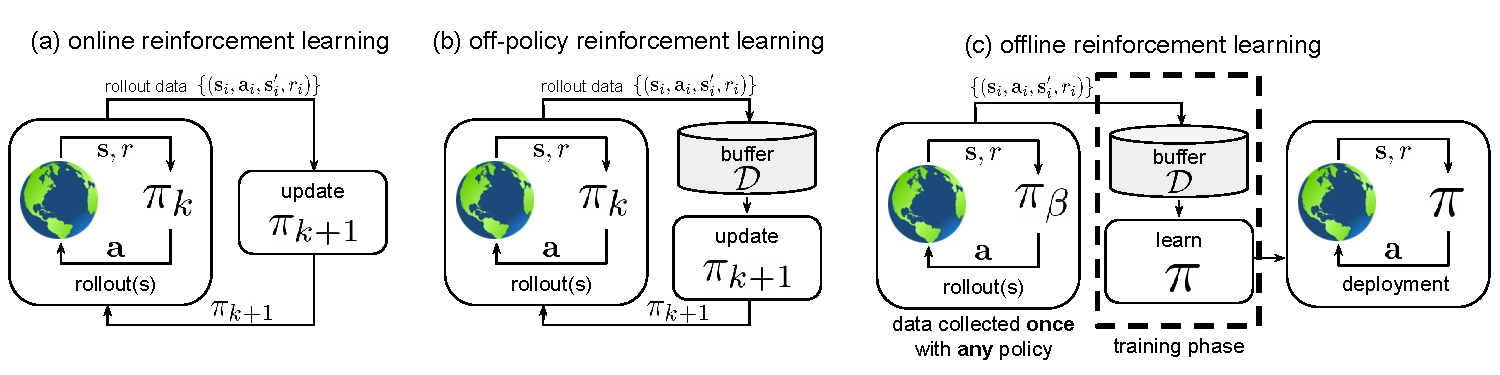
\includegraphics[height=1.5in]{figs/offlineRL}
\caption{
  Comparison of online on-policy RL,  online off-policy RL,
  and offline RL.
\figtaken{Figure 1 of \citep{Levine2020offline}}.
\figthanks{Sergey Levine}.
}
\label{fig:offline}
\end{figure}




\keywordDef{Offline reinforcement learning}
(also called \keywordDef{batch reinforcement learning} \cite{Lange2012})
is concerned with learning a reward maximizing
policy from a fixed, static dataset,
collected by some existing policy,
known as the \keywordDef{behavior policy}.
Thus no interaction with the environment is allowed
(see \cref{fig:offline}).
This makes policy learning harder than the online case,
since we do not know the consequences of actions that were not taken
in a given state, and cannot test any such ``counterfactual'' predictions
by trying them.
(This is the same problem as in off-policy RL, which we discussed in
\cref{sec:offpolicy}.)
In addition, the policy will be deployed on new states that it may not have seen,
requiring that the policy generalize out-of-distribution,
which is the main bottleneck for current offline RL methods \citep{Park2024value}.
%We discuss some solution methods below.
%(See also \citep{Bhargava2024} for a recent comparison
%of the methods we will discuss.)

A very simple and widely used offline RL method
is known as \keyword{behavior cloning} or \keyword{BC}.
This amounts to training a policy to predict the observed
output action $a_t$ associated with each observed state $s_t$,
so we aim to ensure $\pi(s_t) \approx a_t$,
as in supervised learning.
This assumes the offline dataset was created by an expert,
and so falls under the umbrella of imitation learning
(see \cref{sec:BC} for details).
By contrast, offline RL methods can leverage suboptimal data.
We give a brief summary of some of these  methods below.
For more details, 
see e.g., \citep{Levine20Offline,Chen2024offlineRL,Cetin2024}.
For some offline RL benchmarks,
see DR4L \citep{Fu20}, RL Unplugged \citep{Gulcehre20},
OGBench (Offline Goal-Conditioned benchmark) \citep{Park2024},
and D5RL \citep{Rafailov2024}.

%A simple extension of BC to the case where
%the offline dataset was generated by policies of variable
%quality is to filter out trajectories with low reward;
%this is called \keywordDef{filtered BC}.




%For an experimental comparison of
%offline RL methods, see e.g., \citep{Gulcehre20,Fu20,Bhargava2024,Cetin2024}.
%For a more recent approach,
%known as \keywordDef{perceiver actor critic},
%see \citep{Springenberg2024}.


\subsection{Offline model-free RL}


In principle, we can tackle offline RL using the off-policy methods
that we discussed in \cref{sec:offpolicy}.
These use some form of importance sampling, based on
$\policytgt(a|s)/\behavior(a|s)$, to reweight the data in the replay buffer $\data$,
which was collected by 
the behavior policy, towards the current policy (the one  being evaluated/ learned).
Unfortunately, such methods only work well if the behavior policy is
is close to the new policy. In the online RL case,
this can be ensured by gradually updating the new policy away from
the behavior policy, and then sampling new data  
from the updated policy (which becomes the new behavior policy).
Unfortunately, this is not an option in the offline case.
Thus we need to use other strategies to control the discrepancy
between the behavior policy and learned policy, as we discuss below.
(Besides the algorithmic techniques we discuss,
another reliable way to get better offline RL performance
is to train on larger, more diverse datasets,
as shown in \citep{Kumar2023offline}.)

\eat{
Various methods have been developed to control the variance
of the importance weights in the offline case,
as discussed in \citep[Sec 4]{Levine20Offline},
but such methods are not widely used in practice.
}

\subsubsection{Policy constraint methods}

In the \keywordDef{policy constraint} method,
we use a modified form of  actor-critic,  which, at iteration $k$,
uses an update of the form
\begin{align}
  Q^{\pi}_{k+1} &\leftarrow \argmin_Q \expectQ{
    \left(Q(s,a) - (R(s,a) + \gamma \expectQ{Q^{\pi}_k(s',a')}{\pi_k(a'|s')})
    \right)^2
  }{(s,a,s') \sim \data} \\
  \pi_{k+1} &\leftarrow \argmax_{\pi} \expectQ{
    \expectQ{Q^{\pi}_{k+1}(s,a)}{\pi(a|s)}}{s \sim \data}
  \myst D(\policy, \behavior) \leq \epsilon
  \label{eqn:piUpdate}
\end{align}
where $D(\policy(\cdot|s), \behavior(\cdot|s))$ is a divergence measure
on distributions, such as KL divergence or another $f$-divergence.
This ensures that we do not try to evaluate the $Q$ function
on actions $a'$ that are too dissimilar from those seen
in the data buffer (for each sampled state $s$),
which might otherwise result in artefacts similar
an  adversarial attack.


As an alternative to adding a constraint,
we can add a penalty of
$\alpha D(\policy(\cdot|s), \behavior(\cdot|s))$
to the target $Q$ value and the actor objective,
resulting in the following update:
\begin{align}
  Q^{\pi}_{k+1} &\leftarrow \argmin_Q \expectQ{
    \left(Q(s,a) - (R(s,a) + \gamma \expectQ{Q^{\pi}_k(s',a')
    -\alpha \gamma D(\pi_k(\cdot|s'), \behavior(\cdot|s'))}{\pi_k(a'|s')})
    \right)^2
  }{(s,a,s') \sim \data} \\
  \pi_{k+1} &\leftarrow \argmax_{\pi} \expectQ{
    \expectQ{Q^{\pi}_{k+1}(s,a)}{\pi(a|s)}
  - \alpha D(\pi(\cdot|s'), \behavior(\cdot|s'))}{s \sim \data}
\end{align}

One problem with the above method is that we have to fit
a parametric model to $\behavior(a|s)$ in order to evaluate the
divergence term. Fortunately, in the case of KL, the divergence
can be enforced implicitly,
as in the \keywordDef{advantage weighted regression}
or \keywordDef{AWR} method of \citep{Peng2019awr},
the \keywordDef{reward weighted regression} method
of \citep{Peters07},
 the \keywordDef{advantage weighted actor critic}
or \keywordDef{AWAC} method of \citep{Nair2020},
the \keywordDef{advantage weighted behavior model}
or \keywordDef{ABM} method of \citep{Siegel2020},
In this approach, we first solve (nonparametrically) for the new policy
under the KL divergence constraint to
get $\overline{\pi}_{k+1}$, and then we project
this into the required policy function class via
supervised regression, as follows:
\begin{align}
  \overline{\pi}_{k+1}(a|s) &\leftarrow \frac{1}{Z}
  \behavior(a|s) \exp\left( \frac{1}{\alpha} Q_k^{\pi}(s,a) \right) \\
  \pi_{k+1} &\leftarrow \argmin_{\pi} \KLpq{\overline{\pi}_{k+1}}{\pi}
\end{align}
In practice the first step can be implemented by weighting
samples from $\behavior(a|s)$ (i.e., from the data buffer)
using importance weights given by
$\exp\left( \frac{1}{\alpha} Q_k^{\pi}(s,a) \right)$,
and the second step can be implemented via  supervised
learning (i.e., maximum likelihood estimation) using
these weights.

It is also possible to replace the KL divergence
with an integral probability metric (IPM),
such as the maximum mean discrepancy (MMD) distance,
which can be computed from samples,
without needing to fit a distribution $\behavior(a|s)$.
This approach is used in 
\citep{Kumar2019off}.
% https://bair.berkeley.edu/blog/2019/12/05/bear/
This has the advantage that it can constrain the support of the learned
policy to be a subset of the behavior policy,
rather than just remaining close to it.
To see why this can be advantageous, consider the case where
the behavior policy is uniform.
In this case, constraining the learned policy to remain close (in KL divergence)
to this distribution could result in suboptimal behavior,
since the optimal policy may just want to put all its mass on a single action
(for each state).

\subsubsection{Behavior-constrained policy gradient methods}

Recently a class of methods has been developed that is simple and effective:
we first learn a baseline policy $\pi(a|s)$ (using BC) and a Q function
(using Bellman minimization) on the offline data,
and then update the policy parameters to pick actions that have high expected
value according to $Q$ and which are also likely under the BC prior.
%which we call behavior-regularized PG \citep{Wu2020}.
An early example of this is the $Q^{\dagger}$ algorithm
of \citep{Fujimoto2019batch}.
In  \citep{Fujimoto2021}, they present
 the \keywordDef{DDPG+BC} method,
which optimizes
\be
\max_{\pi} J(\pi) = \expectQ{
  Q(s,\mu^{\pi}(s)) + \alpha \log \pi(a|s)}{(s,a) \sim \data}
\ee
where $\mu^{\pi}(s) = \expectQ{a}{\pi(a|s)}$ is the mean of
the predicted action, and $\alpha$ is a hyper-parameter.
As another example,
the \keywordDef{DQL} method of \citep{Wang2023DQL}
optimizes a diffusion policy using
\be
\min_{\pi} \loss(\pi)
= \loss_{\text{diffusion}}(\pi) + \loss_{q}(\pi)
= \loss_{\text{diffusion}}(\pi) 
- \alpha \expectQ{Q(s,a)}{s \sim  \data,
  a \sim \pi(\cdot|s)}
\ee
Finally, \citep{Agarwal2022} discusses how to transfer
the policy from a previous agent to a new agent
by combining BC with Q learning.

\subsubsection{Uncertainty penalties}
\label{sec:offlineUncertainty}

An alternative way to avoid picking out-of-distribution actions,
where the $Q$ function might be unreliable,
is to add a penalty term to the $Q$ function based on the estimated
epistemic uncertainty, given the dataset $\data$,
which we denote by $\text{Unc}(P_D(Q^{\pi}))$,
where $P_D(Q^{\pi})$ is the distribution over $Q$ functions,
and $\text{Unc}$ is some metric on distributions.
For example, we can use a deep ensemble to represent the distribution,
and use the variance of $Q(s,a)$ across ensemble members as
a measure of uncertainty.
%as in \citep{Kumar2019off}.
This gives rise to the following policy improvement update:
\begin{align}
  \pi_{k+1} &\leftarrow \argmax_{\pi} \expectQ{
    \expectQ{
      \expectQ{Q^{\pi}_{k+1}(s,a)}{P_D(Q_{k+1}^{\pi})}
    }{\pi(a|s)}
    - \alpha \text{Unc}(P_D(Q_{k+1}^{\pi}))
}{s \sim \data}
\end{align}
For examples of this approach, see e.g.,
\citep{An2021,Wu2021unc,Ghasemipour2022}.

\subsubsection{Conservative Q-learning and pessimistic value functions}
\label{sec:CQL}
% Sergey Levine talk 2024
% https://www.youtube.com/watch?v=Az5BoT7lCYo&list=PLEA9Mnr-L18lI_I-EkyAc1-gXgBj52oV5


An alternative to explicitly estimating uncertainty
is to add a \keywordDef{conservative penalty}
directly to the $Q$-learning error term.
That is, we minimize the following wrt $\vw$
using each batch of data $\calB$:
\be
\overline{\calE}(\calB,\vw)
   = \alpha \calC(\calB,\vw) + \calE(\calB, \vw)
\ee
where $\calE(\calB, \vw) = \expectQ{ (Q_{\vw}(s,a) -
  (r+\gamma \max_{a'} Q_{\vw}(s',a')))^2}{(s,a,s') \in \calB}$
is the usual loss for $Q$-learning,
and $\calC(\calB,\vw)$ is some conservative penalty.
In the \keywordDef{conservative Q learning}
or \keywordDef{CQL} method of \citep{CQL},
we use the following penalty term:
\be
\calC(\calB,\vw)
= \expectQ{Q_{\vw}(s,a)}{s \sim \calB, a \sim \pi(\cdot|s)}
- \expectQ{Q_{\vw}(s,a)}{(s,a) \sim \calB}
\ee
If $\pi$ is the behavior policy, this penalty becomes 0.

 
\eat{
A natural approach to offline RL is to just perform
Q-learning on the fixed dataset,
and then to compute the policy using
$\pi(a|s) = \argmax_a Q(s,a)$.
In principle this should work, since Q-learning is off-policy,
but in practice it does not work.
The reason is that Q-learning is trying to learn
the optimal policy $\pi^*$, but the data was generated by
a fixed \keyword{behavior policy}
$\pi_{\beta}$, so when Q-learning predicts the value
of the best action, it cannot be checked against the data,
and it might become over optimistic.



To see this in more detail, let us rewrite
the Bellman backup in terms of a distribution
$\pi_{\tnew}$ that puts all its mass on the optimal action
(according to the current $Q$) for each state,
so $\pi_{\topt}(a|s)=\delta(a-\argmax_{a'} Q(s,a'))$.
Thus the TD loss becomes
\be
J_{\beta}(Q,\pi) = \expectQ{ (Q(s,a)-\targetV(s,a))^2}{\pi_{\beta}(s,a)}
\ee
where the target $\targetV(s,a)$ is defined by 
\be
\targetV(s,a) =
  r(s,a) + \expectQ{Q(s',a')}
  {\pi_{\beta}(s') \pi_{\topt}(a'|s')}
\ee
If we have $\pi_{\beta}(s,a)=\pi_{\beta}(s) \pi_{\topt}(s|a)$, this optimization
should work well, since the training data comes
from the optimal distribution, and thus we have a stable system.
But for suboptimal behavior data, Q-learning will learn
to find actions that do better than the training data,
according to $Q$; this is like finding adversarial examples
for a network, and can result in unstable behavior,
where the estimated $Q$ values increase, but the actual reward
decreases.

% Pessimism-based methods eg CQL
% Policy constraints (eg BRAC)
% Avoid OOD actions in updates (eg AWAC, IQL). Don't evaluate
%  actions you didn't train on.

One way to deal with the overestimation problem is to use
 \keywordDef{conservative Q learning}
 or \keywordDef{CQL} \citep{CQL}.
The idea is to find $(s,a)$ points where the
$Q$-function might be overestimating the true value,
and then to ``push down'' on the estimate,
so it becomes more conservative.
In practice this amounts to adding the following
regularizer (scaled by $\alpha$) to $J_{\beta}$:
\begin{align}
J_{CQL}(Q,\pi)
&=   \expectQ{ Q(s,a) -\expectQ{Q(s,a')}{a' \sim \pi(\cdot|s)}
}{(s,a) \sim \data} \\
&=  \expectQ{Q(s,a)}{(s,a) \sim \data}
- \expectQ{Q(s',a')}{s' \sim \data, a' \sim \pi(\cdot|s')}
\label{eqn:CQL}
\end{align}
%The first term in the regularizer pushes down on all
%$Q$ values, whereas the second term pushes up on
%the $Q$ values encountered in the data.
%One can prove that
%$\hat{Q}^{\pi} \leq Q^{\pi}$ for large enough $\alpha$.
%The $\alpha$ coefficient determines the strength of this
%regularization.


}

 \eat{
the approach attempts to generalize beyond  offline data,
but not too far.
First it uses Q learning to solve
\be
\argmin_{\vw} [Q_{\vw}(s_t,a_t) - \expectQ{r(s_t,a_t) + Q_{\vw}(s_{t+1},a_{t+1})}{\pemp}]^2
\ee
where $\pemp$ is the empirical distribution over trajectories.
It also fits the BC policy $q_{\beta}(a_t|s_t)$.
Finally  it finds the policy that is closest
(in the chosen parametric family)
to
$q(a_t|s_t) \propto \exp(Q_{\vw}(s_t,a_t) q_{\beta}(a_t|s_t))$,
which is the BC policy weigthed  by the Q function.
It does this by solving a weighted MLE problem
\be
\argmin_{\vtheta} \KLpq{\pi_{\vtheta}(a_t|s_t)}{q(a_t|s_t)}
\ee
%
 }


     
\subsection{Offline model-based RL}
\label{sec:offlineMBRL}


In \cref{sec:MBRL}, we discussed model-based RL,
which can train a dynamics model given a fixed dataset,
and then use this to generate synthetic data
to evaluate and then optimize  different possible policies.
However, if the model is wrong, the method may learn a suboptimal
policy, as we discussed in \cref{sec:modelUncertainty}.
This problem is particularly severe in the offline RL case,
since we cannot recover from any errors by collecting more data.
Therefore various conservative MBRL algorithms have been developed,
to avoid exploiting model errors.
For example, \citep{Kidambi2020} present the
\keywordDef{MOREL} algorithm,
and \citep{Yu2020mopo} present the \keywordDef{MOPO} algorithm.
Unlike the
value function uncertainty method of \cref{sec:offlineUncertainty},
or the conservative value function method of \cref{sec:CQL},
these model-based methods add a penalty for visiting states where
the model is likely to be incorrect.

In more detail, let $u(s,a)$ be an estimate of the uncertainty of the
model's predictions given input $(s,a)$.
In MOPO, they define a conservative reward using
$\overline{R}(s,a) = R(s,a) - \lambda u(s,a)$,
and in MOREL, they modify the MDP so that the agent enters an
absorbing state with a low reward when $u(s,a)$ is sufficiently
large.
In both cases, it is possible to prove that the model-based
estimate of the policy's performance under the modified
reward or dynamics is a lower bound of the performance
of the policy's true performance in the real MDP,
provided that the uncertainty function $u$ is an error oracle,
which means that is satisfies
$D(M_{\vtheta}(s'|s,a), M^*(s'|s,a)) \leq u(s,a)$,
where $M^*$ is the true dynamics, and $M_{\vtheta}$
is the estimated dynamics.

For more information on offline MBRL methods,
see \citep{Chen2024offline}.



 
\subsection{Offline RL using reward-conditioned sequence modeling}
\label{sec:seqModel}

Recently an approach to offline RL
based on sequence modeling has become very popular.
The basic idea --- known as \keywordDef{upside down RL}
\citep{Schmidhuber2019}
or \keywordDef{RvS} (RL via Supervised learning)
\citep{Kumar2019,Emmons2021} ---
is to train a generative model over future states
and/or actions conditioned on the observed reward,
rather than predicting the reward given a state-action
trajectory.
%This reduces to a supervised learning problem
%(albeit with high dimensional output).
At test time, the conditioning is changed
to represent the desired reward, and futures
are sampled from the model.
The implementation of this idea then depends on what
kind of generative model to use, as we discuss below.

The \keywordDef{trajectory transformer}
method of \citep{trajectoryTransformer}
learns a joint model of the form
$p(\vs_{1:T}, \va_{1:T}, \vr_{1:T})$
using a transformer,
and then samples from this using beam search,
selecting the ones with high reward (similar to MPC, \cref{sec:MPC}).
The \keywordDef{decision transformer} \citep{decisionTransformer}
is related, but  just generates action sequences,
and conditions on the past observations and the future reward-to-go.
That is, it fits
\be
\argmax_{\vtheta} \expectQ{
  \log \pi_{\vtheta}(a_t|s_{0:t}, a_{0:t-1}, \text{RTG}_{0:t})}{\pemp}
\ee
where $\text{RTG}_t = \sum_{k=t}^T r_t$ is the return to go.
(For a comparison of decision transformers to other offline RL methods,
see \citep{Bhargava2024}.)

The \keywordDef{diffuser} method of \citep{diffuser}
is a diffusion version of trajectory transformer,
so it fits $p(\vs_{1:T}, \va_{1:T}, \vr_{1:T})$ using diffusion,
where the action space is assumed to be continuous.
They also replace beam search with classifier guidance.
The \keywordDef{decision diffuser} method of \citep{decisionDiffuser}
extends diffuser by using classifer-free guidance,
where the conditioning signal is the reward-to-go,
simlar to decision transformer.
However, unlike diffuser,
the decision diffuser just models the future state trajectories
(rather than learning a joint distribution over states and actions),
and infers the actions using an \keywordDef{inverse dynamics model}
$a_t = \pi(s_t, s_{t+1})$,
which is trained using supervised learning.

One problem with the above approaches is that conditioning
on a desired return and taking the predicted action can fail dramatically
in stochastic environments,
since trajectories that result in a return may have only
achieved that return due to chance \citep{Paster2022,Yang2023,Brandfonbrener2022,Villaflor2022}.
(This is related to the optimism bias in the control-as-inference
approach discussed in \cref{sec:RLAI}.)

 
\subsection{Hybrid offline/online methods}

Despite the progress in offline RL, it is fundamentally
more limited in what it can learn compared to online RL
\citep{Ostrovski2021}.
Therefore, various hybrids of offline and online RL have been proposed,
such as
\citep{Ball2023} and \citep{Nakamoto2023}.

For example,
\citep{Nakamoto2023}
suggest pre-training
with offline RL (specifically CQL) followed by online finetuning.
Naively this does not work that well, because CQL can be
too conservative, requiring the online learning
to waste some time at the beginning fixing
the pessimism. So they propose a small
modification to CQL,
known as \keywordDef{calibrated Q learning}.
This simply prevents CQL from being too conservative,
by replacing the CQL
regularizer
%in \cref{eqn:CQL}
with
\be
\min_Q \max_{\pi}
J(Q,\pi)    + \alpha  \expectQ{
  \max(Q(s,a), V^{\pi_{\beta}}(s))
  - \alpha \expectQ{Q(s,a)}{(s,a) \sim \data}
}{s \sim \data, a \sim \pi(a|s)}
\label{eqn:CalQL}
\ee
where the $Q(s,a)$ term inside the $\max$
ensures conservatism (so $Q$ lower bounds
the value of the learned policy),
and the $V^{\pi_{\beta}}(s)$ term
ensures ``calibration''
(so $Q$ upper bounds the value
of the behavior policy).
Then online finetuning is performed in the usual way.

%This seems like a promising practical solution
%for creating RL systems that work in the real-world.





\section{Extreme-token Phenomena in pretrained LLMs} \label{sec:llm}

%\DP{TODO for SONG: rewrite this paragraph}
% \DP{TODO for DRUV: check again after Song finishes}

In this section, we investigate extreme-token phenomena in open-source pretrained LLMs. In \Cref{sub:active_dormant}, we analyze the static behavior of these phenomena in Llama 2-7B-Base \citep{touvron2023llama}, confirming the existence of the \textit{active-dormant mechanism} in LLMs. Notably, we identify a specific head that is active on GitHub samples but dormant on Wikipedia samples. In \Cref{sub:olmo_dynamics}, we examine the dynamic behavior of extreme-token phenomena during the pretraining of OLMo-7B \citep{groeneveld2024olmo}. We show that the attention logits, value states norm, and residual states norm of the sink token(s) in OLMo reflect behavior similar to that of the simpler BB model. Specifically, the simultaneous formation of attention sinks and value-state drains gives evidence for the \textit{mutual reinforcement mechanism}.

% It turns out that our exploration into the BB task in \Cref{sec:bb_task} may actually shed light upon the origin of attention sinks, small value states, and massive norms in full-fledged large language models trained on massive amounts of text. To verify this claim, we once again summarize and elaborate the observations we made in the BB task model:
% \begin{enumerate}[leftmargin=2em]
% \setlength\itemsep{0pt}
%     \item The attention sinks and value-state drains are external manifestations of the active-dormant mechanism in LLMs. 
%     \item The lower-layer components (e.g., attentions and MLPs) of the LLM contribute to all three extreme-token phenomena.     
%     \item The attention heads go through the attention-increasing and value-state-shrinking phase. They converge to the stable phase, with identical attention logits on the \bos~token. Meanwhile, the residual state norm corresponding to the \bos{} token linearly increase during pretraining.
% \end{enumerate}

% We will confirm each of these observations in this section.\footnote{Here, we mention that in order to achieve this checklist, we had to do a certain amount of translating from the setting of the BB model to the setting of LLMs. For example, the BB model identifies trigger tokens as the (semantically) important tokens in that the model should change behavior after seeing them. In the context of LLMs, almost every token fits this description for a suitable context, but tokens like \bos{} do not. 
% %\tianyu{I think we should say that each token could be trigger or non-trigger, depending on the context? If every tokens are triggers, there's no dormant phase.}
% } Namely, in \Cref{sub:active_dormant} we will confirm point 1; in \Cref{sub:circuits} we confirm point 2; and in \Cref{sub:olmo_dynamics} we confirm point 3.


\subsection{Active-dormant mechanism in LLMs}\label{sub:active_dormant}


\begin{figure}
    \centering
    \begin{subfigure}[t]{0.58\textwidth}
        \centering
        \caption{\small Attention weights for GitHub/Wikipedia data}% \sm{Maybe 2 by 2? }}
        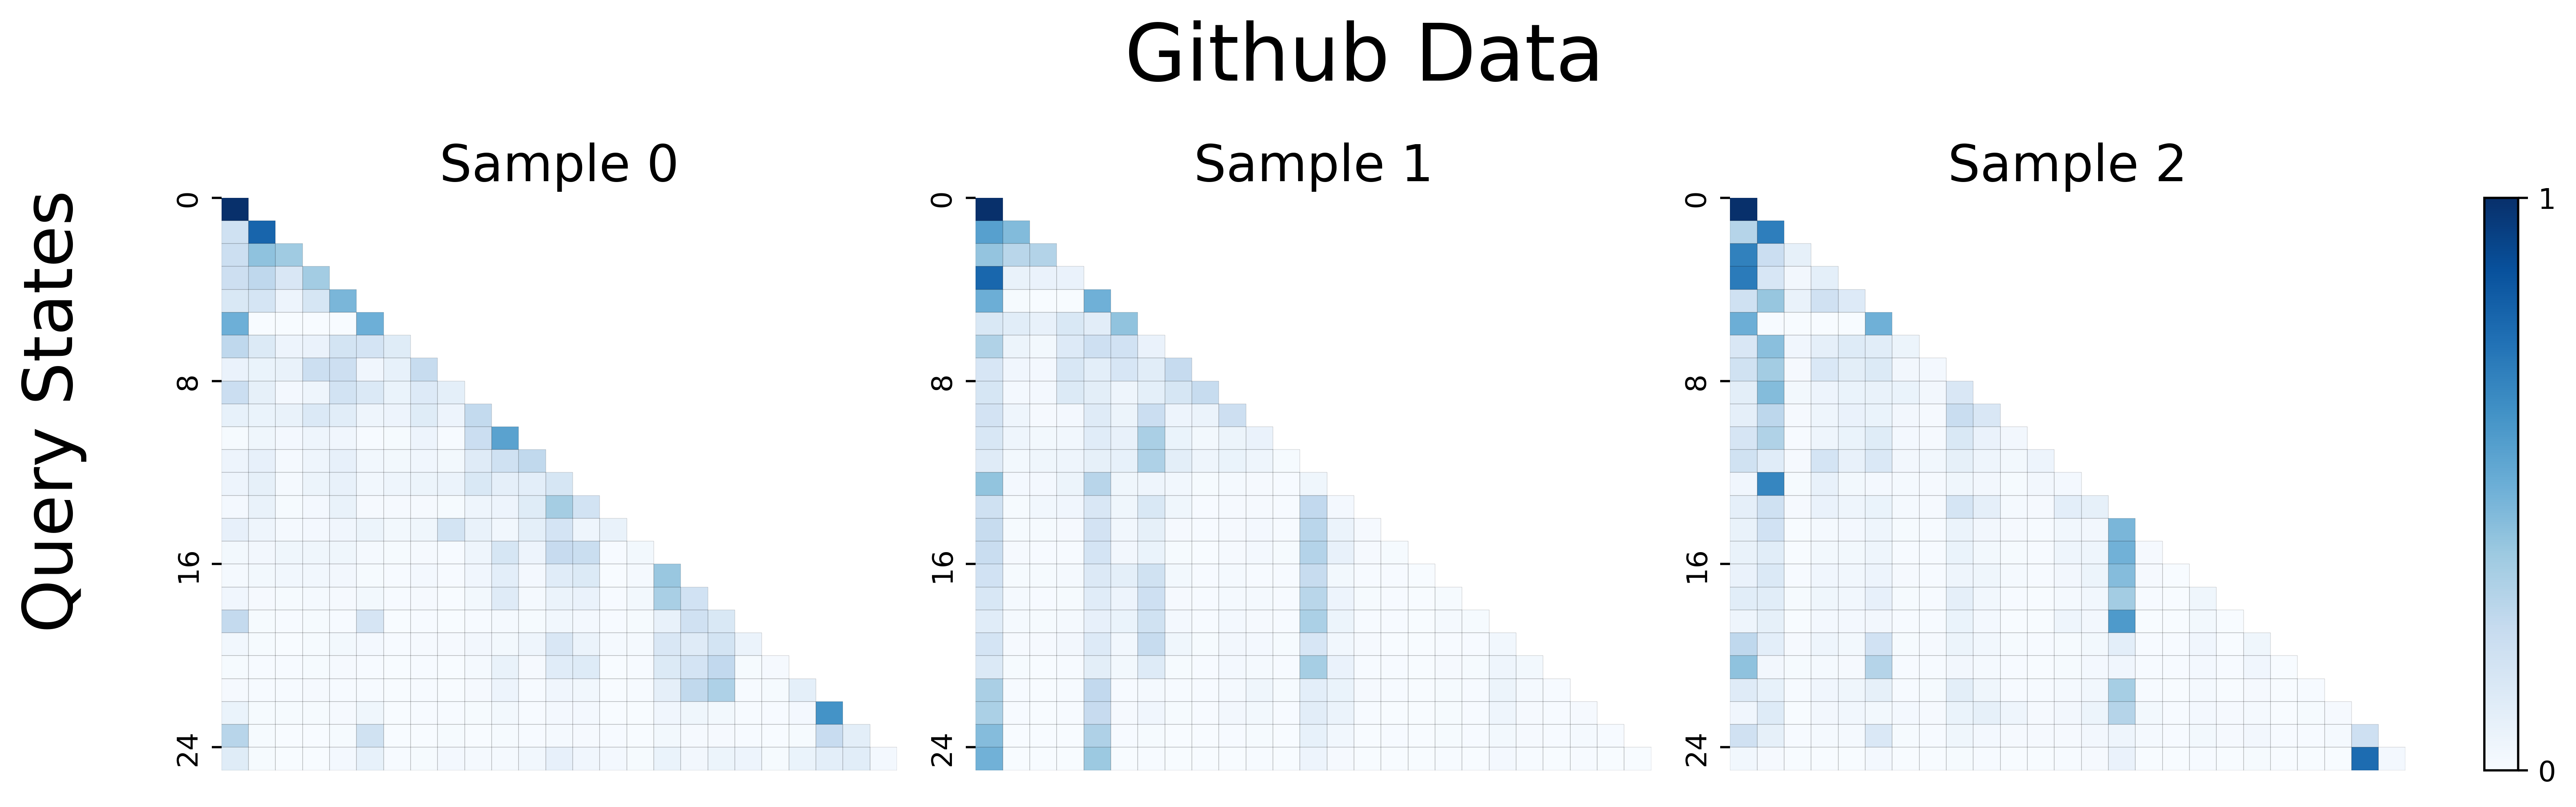
\includegraphics[width=0.9\textwidth]{Figures/L16_H25/attn_github_head25.png}
        
        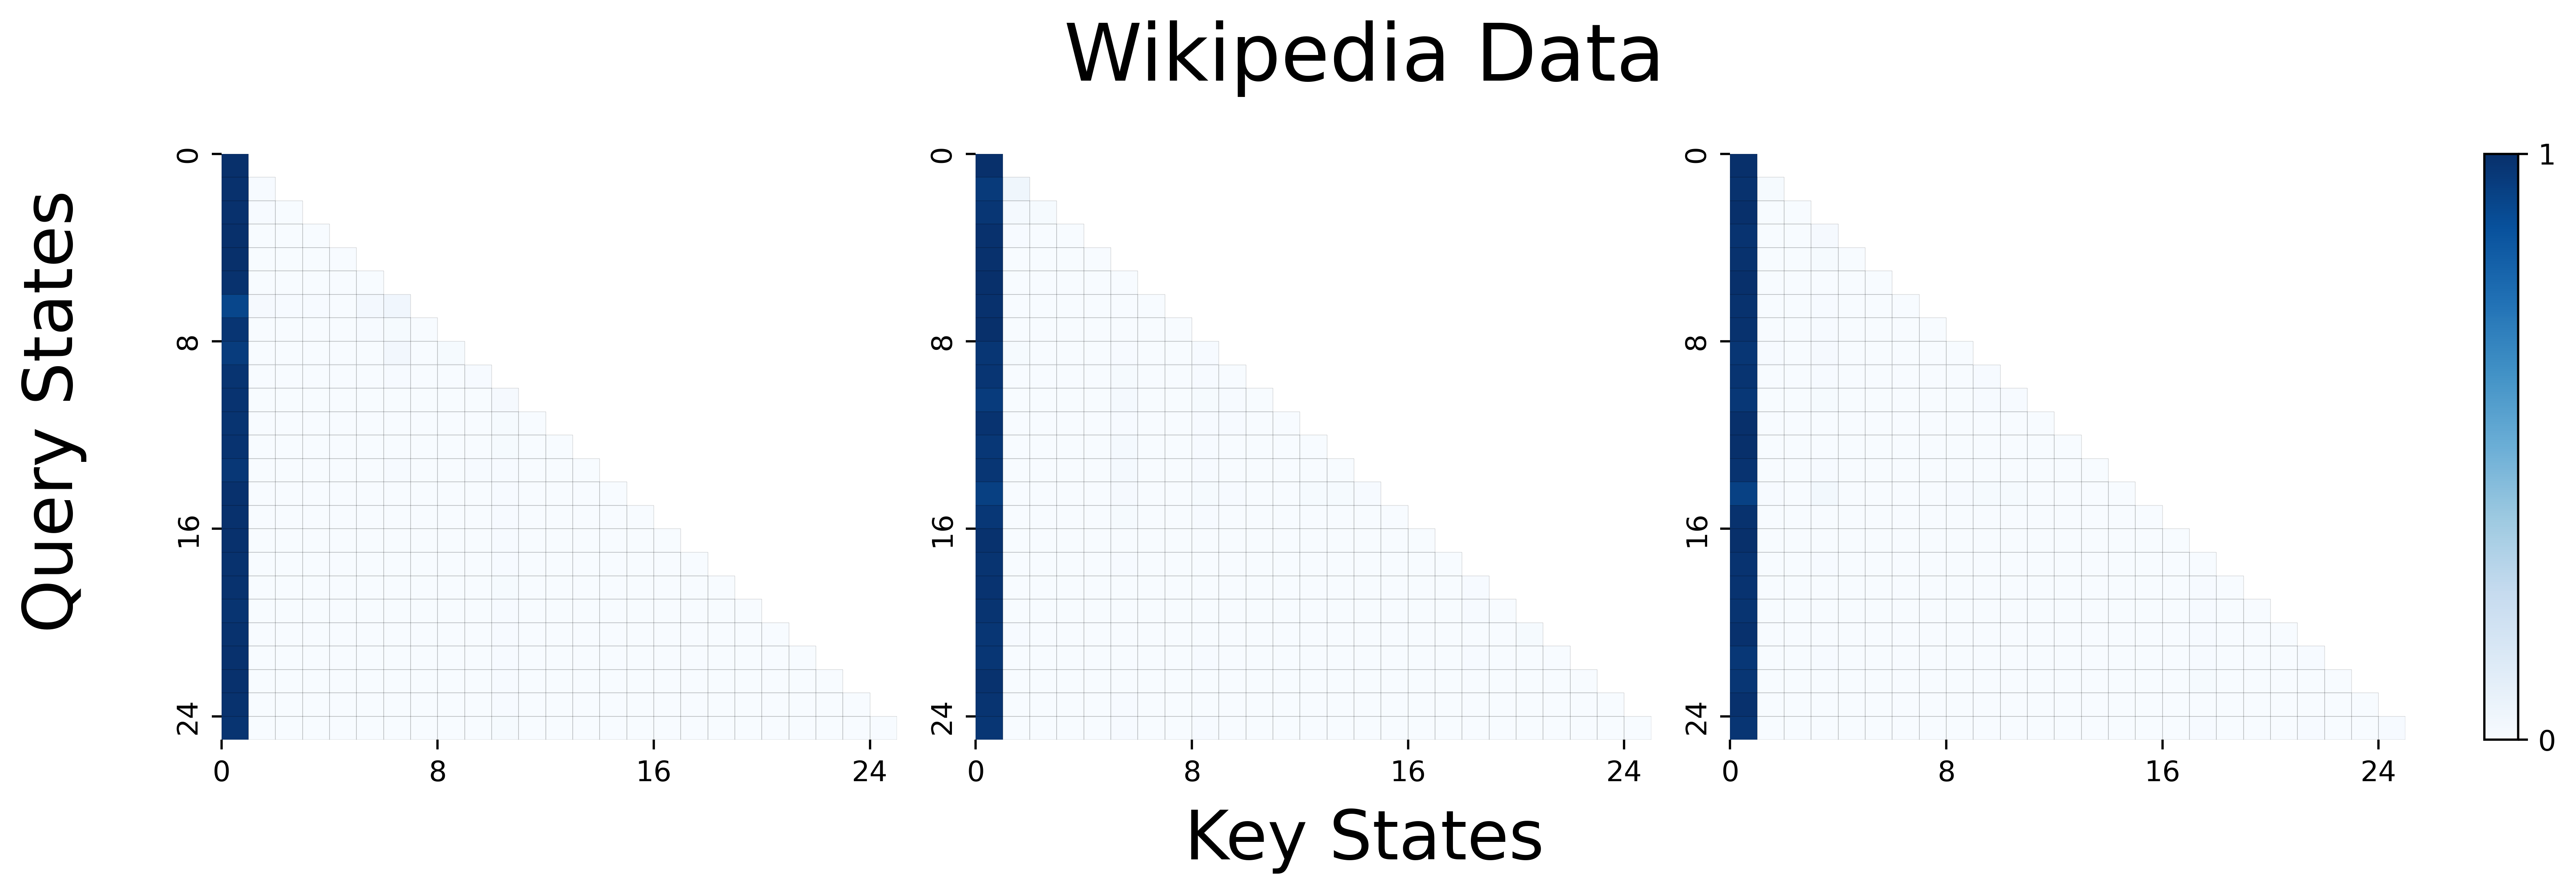
\includegraphics[width=0.9\textwidth]{Figures/L16_H25/attn_wikipedia_head25.png}
        \label{fig:github_wikipedia_weights}
    \end{subfigure}
    \hfill
    \begin{subfigure}[t]{0.38\textwidth}
        \caption{\small Zero-out-head intervention outcomes}
        \label{fig:github_wikipedia_zero_out}
        \vskip1.5em
        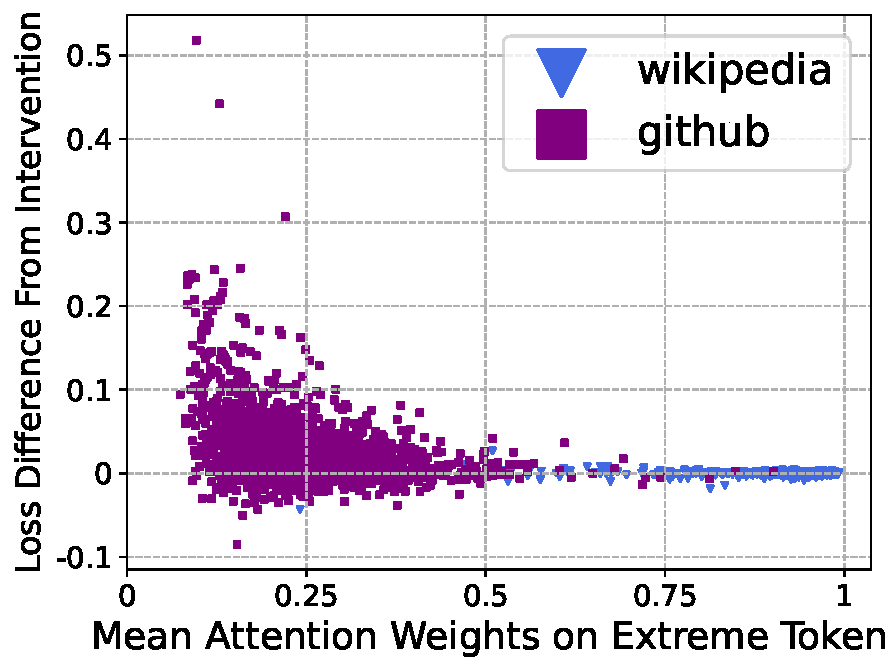
\includegraphics[width=0.9\textwidth]{Figures/BBM/LLM_interventions.pdf}
    \end{subfigure}
    \vspace{-0.5em}
    %\includegraphics[width=0.5\linewidth]{}
    \caption{\small \textbf{Active-dormant mechanism of Layer 16 Head 25 (L16H25) of Llama 2-7B-Base.} We observe that L16H25 is active on GitHub data and dormant on Wikipedia data, both sourced from RedPajama-1T \citep{together2023redpajama}. \textit{Left (a)}: Attention weights of L16H25, prompted by three randomly selected samples from each domain. \textit{Right (b)}: Results of an intervention study showing the change in cross-entropy loss when the output of L16H25 (specifically, its value states) is set to zero across sequences in both domains. The findings indicate that the model's performance for GitHub data, measured by cross-entropy loss, strongly relies on the output of this attention head. 
    % \sm{(a) Truncate at $24$ \sm{right: xlabel and xtick size. $x 0.1$} \sm{High priority} \sm{Orange color change}}
    % heads are sinks in one domain and not others (Llama 2 7B L16H25, GitHub vs Wikipedia) \DP{TODO...}
    % \DP{Plan: two figures. Left: attn sink visualization for GitHub on left and Wikipedia (4x4 (adjust to be visually appealing) samples visualize L16H25). Right: causal intervention, zeroing out head vs cross entropy delta taken across many samples from GitHub and Wikipedia.}
    }
    \label{fig:dormant_heads_domain_dependent}
\end{figure}




    %\textit{If all tokens at a head do not have helpful value states for predicting the next token, then attention mass will concentrate on tokens which are generally unhelpful for next-token prediction (like \bos). \sm{Attention heads are controlled by the active-dormant mechanism; attention sinks and value-state drains are the dormant phases of attention heads. }}

Our study of the BB model leads to the following prediction with respect to the extreme-token phenomena, which we hypothesize also applies to LLMs:  
\begin{center}
    \textit{Attention heads are controlled by an active-dormant mechanism (cf.\ Claim \ref{claim:active-dormant}). The presence of attention sinks and value-state drains indicates that an attention head is in a dormant phase.}
\end{center}

This hypothesis suggests that in LLMs, whether an attention head becomes a sink depends on the context. Specifically, the attention head may become entirely irrelevant for selecting the next tokens in certain contexts or tasks, but not in others. When this irrelevance occurs, the attention head transitions into an attention sink. This hypothesis was confirmed in small transformers and the BB task, as demonstrated in Section~\ref{sec:bb_task}. 



Accordingly, we aim to identify instances of attention heads in pretrained LLMs that exhibit this active-dormant behavior, i.e., heads that are dormant in some domains but active in others. In \Cref{fig:dormant_heads_domain_dependent}, we display a particular attention head---Layer 16 Head 25 (L16H25) of Llama 2-7B-Base \citep{touvron2023llama}---which demonstrates a clear active-dormant distinction across two distinct contexts (e.g., tokens from the GitHub subset versus the Wikipedia subset of RedPajama \citep{together2023redpajama}). While many attention heads show similar context-dependent behavior (see \Cref{sec:more_heads}), we focus on this one because the conditions for its activation are straightforward and interpretable, whereas other heads may have more nuanced criteria. 
% \sm{Can we plot more figures instead of the figures that are GitHub/Wiki}

\Cref{fig:github_wikipedia_weights} shows the attention maps of L16H25 on samples from both the GitHub and Wikipedia subsets of RedPajama. It demonstrates that L16H26 is \textit{dormant} (i.e., an attention sink) on samples from Wikipedia, which resemble prose, and \textit{active} (i.e., not an attention sink) on samples from GitHub, which resemble code. Additionally, \Cref{fig:github_wikipedia_zero_out} compares the loss difference when L16H25 is zeroed out for prompts from both domains. The results show that zeroing out this head significantly decreases model performance on GitHub sequences, while having minimal impact on Wikipedia sequences. This observation also confirms the head behaves as dormant in some contexts and active in others---in some contexts, removing this head has no effect on model performance, while in others, its removal causes significant performance drops.
% We include more detail in \Cref{sec:circuit}.
% , where we extract a circuit for extreme-token phenomena to examine the dormant-active mechanism and its interaction with input token semantics. \sm{Polish} \sm{Mid priority}



% Accordingly, we strive to find instances of heads in pretrained LLMs that satisfy this principle, i.e., which are dormant on some domains and active on others. In \Cref{fig:dormant_heads_domain_dependent}, we show a particular attention head -- Layer 16 Head 25 of Llama 2-7B-Base \citep{touvron2023llama} --- which has an extremely clear active-dormant distinction across two distinct contexts (e.g., tokens from RedPajama \citep{together2023redpajama} drawn from the GitHub subset versus the Wikipedia subset). While there are many such attention heads which are context-dependent --- we provide some in \Cref{sec:more_heads} --- we demonstrate this one because the conditions under which it is active are simple and interpretable, while others have more involved or complex criteria to become active. We observe that this attention head is \textit{dormant} (i.e., an attention sink) on samples from Wikipedia, which more closely resemble prose, and \textit{active} (i.e., not an attention sink) on samples from GitHub, which more closely resemble code. We also observe that this attention head, in general, contributes significantly to the performance of the model on code sequences, but has negligible impact on the performance of the model on prose sequences (\Cref{fig:github_wikipedia_zero_out}). This is a further justification, from a practical perspective, of why this head is sometimes dormant and sometimes active --- in some contexts we can ablate it from the model entirely with no effect, but in other contexts ablating the head leads to huge performance drops. We include more detail in \Cref{sec:circuit}, where we extract a circuit for extreme-token phenomena in order to analyze the dormant-active mechanism and its interaction with the semantics of the input tokens.

%\footnote{Llama 2-7B-Base has two sink tokens (\bos~and one more) in its attention sink heads, while Llama 3.1-8B-Base only has one (\bos). We discuss a potential reason in \Cref{sub:multiple_sinks_discussion}. \sm{Why we put this remark here?}} \sm{Talk about other heads also has dormant and active phase, though not interpretable. Ablation figures in appendix. } \DP{@SM: the first part is already in the paragraph.} \sm{It would be good to link to figures for other heads. } \DP{sure will add to appendix, and comment out this comments when done}

\subsection{Extreme-token phenomena along training dynamics of LLMs}\label{sub:olmo_dynamics}


\begin{figure}[t]
    \centering
    \begin{subfigure}[t]{0.32\textwidth}
        \centering 
        \caption{\small Attention sink dynamics}
        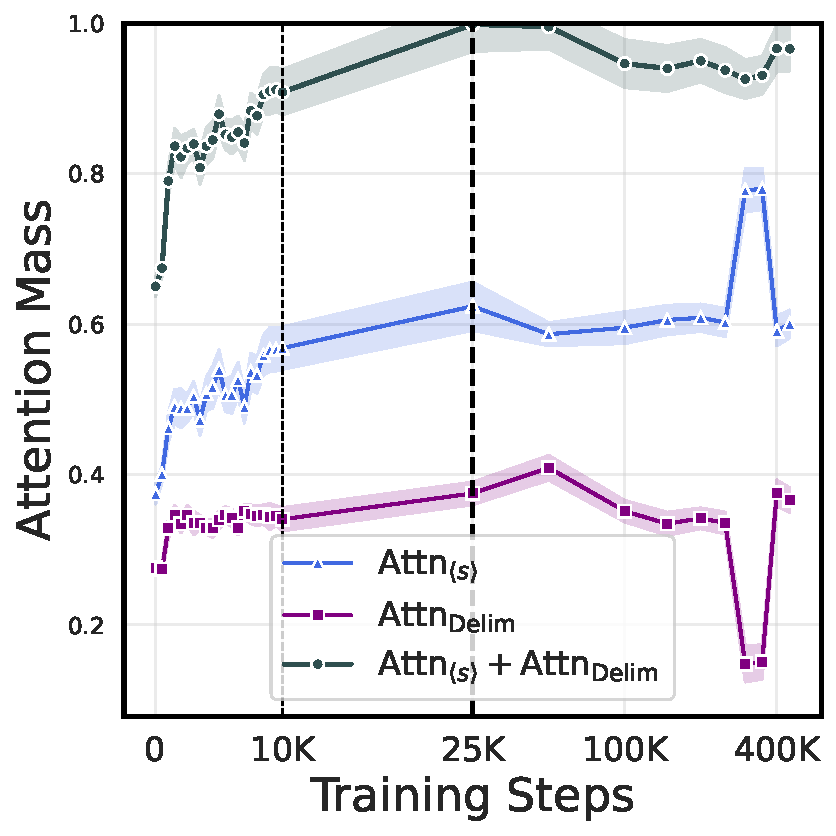
\includegraphics[width=0.9\textwidth]{Figures/olmo/attn_mass_on_top_two_tokens.pdf}
        \label{fig:olmo_sink}
    \end{subfigure}
    \begin{subfigure}[t]{0.32\textwidth}
        \centering 
        \caption{\small Value state dynamics}
        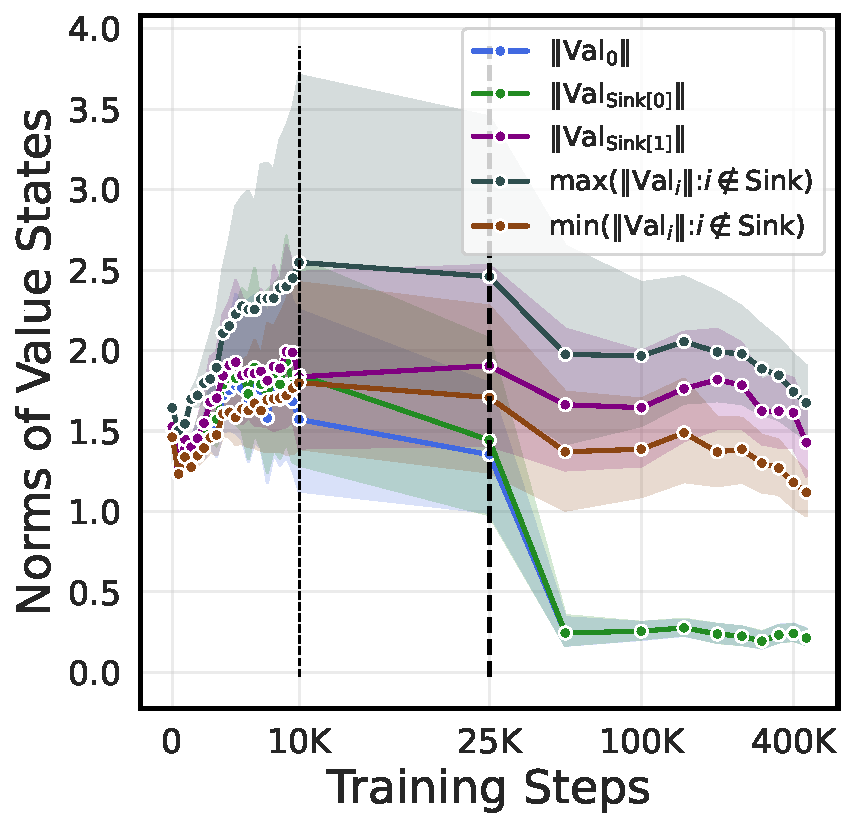
\includegraphics[width=0.9\textwidth]{Figures/olmo/value_norms.pdf}
        \label{fig:olmo_drain}
    \end{subfigure}
    \begin{subfigure}[t]{0.32\textwidth}
        \centering 
        \caption{\small Residual state dynamics}
        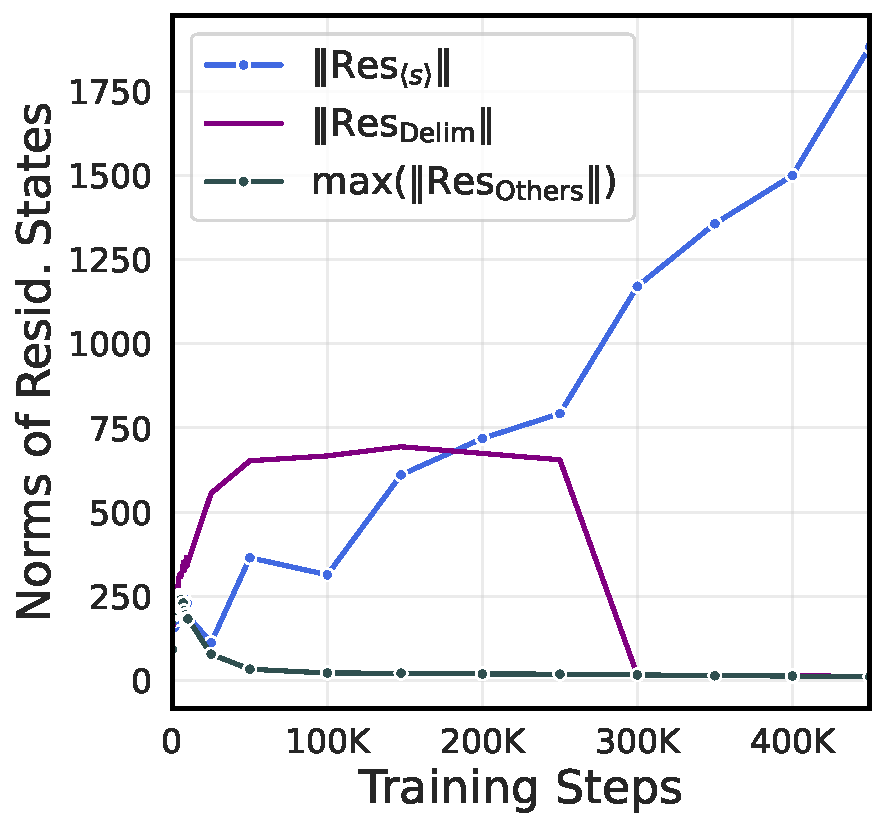
\includegraphics[width=0.9\textwidth]{Figures/olmo/layer_output_norms.pdf}
        \label{fig:olmo_peak}
    \end{subfigure}
    % \vspace{-2em}
    \caption{\small \textbf{Attention weights, value state norms, and residual state norms of Layer 24 during the training dynamics of OLMo.} \textit{Left (a)}: The total attention mass on extreme tokens \bos~and ``\text{Delim}''(\period) at Layer 24, averaged across all attention heads. The horizontal axis is logarithmically scaled after step $10$k. We observe a rapid increase followed by stabilization within the range \([0.9, 1]\) for the rest of training, consistent with our predictions. \textit{Middle (b)}: The value state norms of each token at Layer 24 during training, averaged over all heads. The horizontal axis is logarithmically scaled after step $10k$. Initially, the value states of all tokens shrink, eventually converging, while the value states of the extreme tokens shrink to significantly lower levels compared to other tokens. Figure \textit{(a)} and \textit{(b)} coincide with the trends in Figure~\ref{fig:dynamics} under the BB task. \textit{Right (c)}: The residual state norms of each token at Layer 24 during training. The residual state norm of \bos~increases linearly in magnitude throughout training, matching Figure~\ref{fig:sgd} in the BB task.}
    % \sm{Thicker} \sm{L24 is a bit repetitive} \sm{For (a) and (b), is there a way to draw 0 - 50K using linear scale and 50K - 500K using log scale? This could match better Figure 3(b)} \tianyu{link back to corresponding figures in BB task}}



    
    \label{fig:olmo_predictions_phase0}
\end{figure}
\begin{figure}[h]
    \centering
    \hfill
    \begin{subfigure}[t]{0.32\textwidth}
        \centering 
        \caption{\small Logit dynamics}
        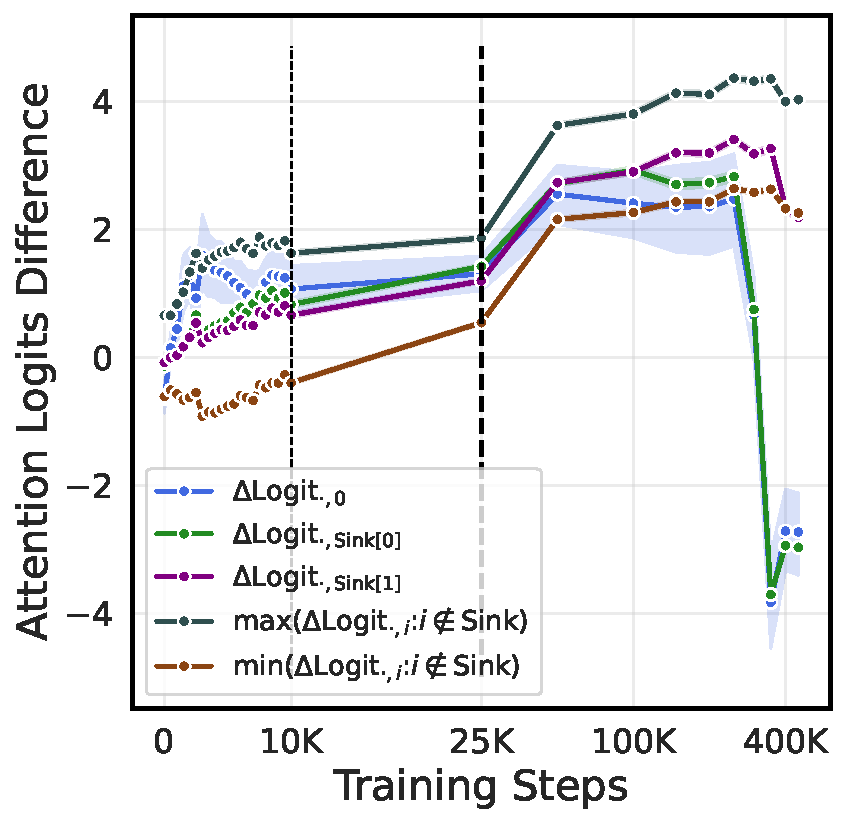
\includegraphics[width=0.9\textwidth]{Figures/olmo/attention_logits.pdf}
        \label{fig:attention_logits_olmo_dynamic}
    \end{subfigure}
    \hfill
    \begin{subfigure}[t]{0.32\textwidth}
        \centering 
        \caption{\small Sink-logits concentration}
        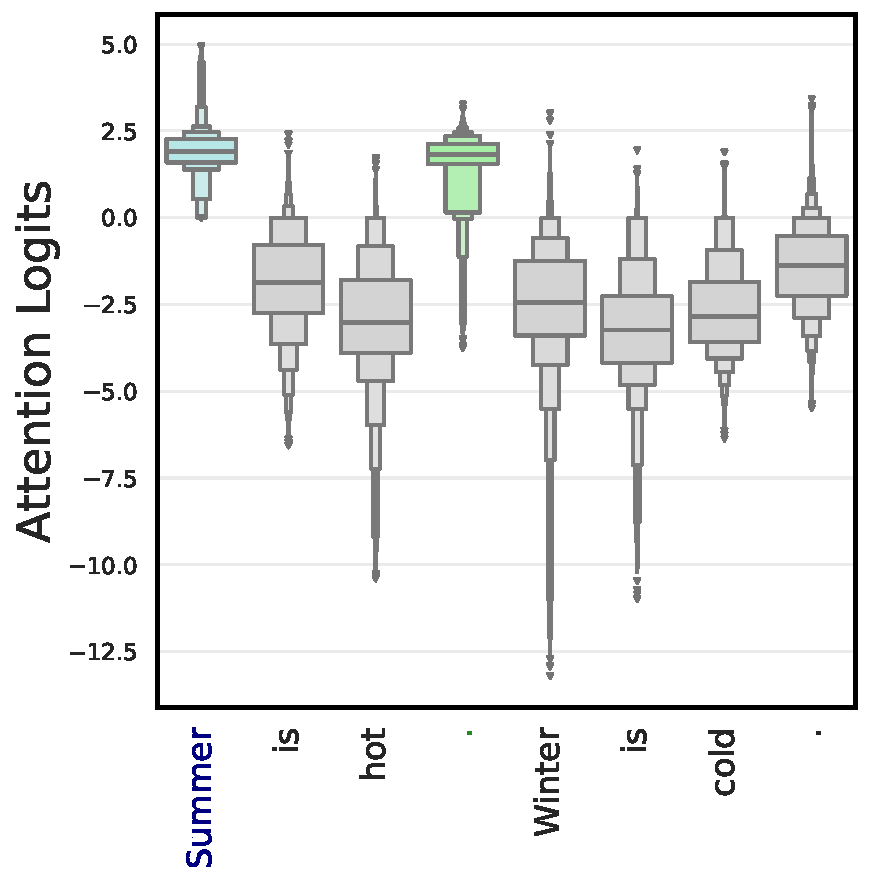
\includegraphics[width=0.9\textwidth]{Figures/olmo/attention_logits_on_test.pdf}
        \label{fig:attention_logits_olmo_static}
    \end{subfigure}
    \hfill
    \phantom{.}
    % \vspace{-2em}
        \caption{\small \textbf{Attention logits of Layer 24.}  \textit{Left (a)}: Attention logits difference of all tokens' query states against \bos's key state during training. The difference in attention logits is computed as \(\Delta\mathrm{logit}_{\cdot,\bos} = \query_{\cdot}^\top \key_{\bos} - \text{Mean}[\query_{\cdot}^\top \key_{\text{Others}}]\). The horizontal axis is logarithmically scaled after step $10k$. We observe that $\Delta \mathrm{logit}_{\cdot,\bos}$ increases approximately in logarithmic scale during training steps $10$k to $100$k, matching the decreasing phase of the value states in Figure~\ref{fig:olmo_drain}. 
        % This behavior aligns with the stable-phase prediction made in the BB model in \Cref{thm:main}(c). Note that this prediction does not apply to the logit corresponding to the zeroth query and key token, as its softmax value will be set to \(1\), making its behavior irrelevant for prediction. 
        \textit{Right (b)}: Attention logits of the last token's query state against all token's key states for pretrained OLMo. In this experiment, we generate \(128\) randomly sampled test tokens with IDs from \(100\) to \(50000\) in the OLMo tokenizer. We append each token separately to the test phrase ``Summer is warm\period~Winter is cold\period'', creating \(128\) different samples, which we feed to the LLM to examine the model behavior. We plot the distribution of (un-shifted) attention logits \( \text{logit}_{\cdot,\tok}=\query_{\mathrm{test}}^\top \key_{\tok}\) across all heads at Layer 24 and all test tokens. The distribution of $\text{logit}_{\cdot,\bos}$ and $\text{logit}_{\cdot,\text{Delim}}$ have considerably small variance compared with other logits, confirming the sink-logits concentration phenomenon. }
        % \tianyu{maybe to make it more clear, we can say that the variance of the attention logits on \bos~is small. Or we can use a new name (attention logits concentration)} \sm{tick size. Box thicker. } \sm{pdf} \tianyu{change the logit in (a)}}
    % \caption{\small \textbf{Attention logits of Layer 24.}  \textit{Left (a)}: The normalized attention logits of all tokens' query states against \bos's key state during training \sm{Is it the opposite?}. We observe that the logits of all non-extreme tokens' query states against \bos's key state in OLMo's Layer 24 are stable for a large fraction of the training run, after an initialization period. This echoes the stable phase prediction made in the BB model in \Cref{thm:main}(c). Note that this prediction makes no guarantees about the logit corresponding to the zeroth query token and zeroth key token, which will be set to \(1\) by the softmax and so its behavior is irrelevant for prediction. Also note that we use normalization, similar to \Cref{sec:bb_task}, to make all terms comparable; namely we have \(\mathrm{logit}_{i} = \langle \query_{i}, \key_{0}\rangle - \mathtt{mean}_{j}(\langle \query_{i}, \key_{j}\rangle)\). \textit{Right (b)}: \sm{A summary phrase of the figure.} For this experiment, we generate \(128\) randomly sampled test tokens with IDs from \(100\) to \(50000\) in the OLMo tokenizer. We append each token separately to the test phrase ``Summer is warm. Winter is cold.'', creating \(128\) different samples, which we feed to the LLM to record the model behavior. We plot the distribution of (un-normalized) dot products \(\langle \query_{\mathrm{test}}, \key_{j}\rangle\) across all heads at Layer 24 and all test tokens. We observe that logits of all regular tokens have very similar distributions, and the distributions of the logits corresponding to extreme tokens \(0\) and \(3\) are also similar. \sm{Why similar? } This confirms the hypothesis that at the end of training, attention heads converge to the stable phase, with similar logits on extreme tokens. \tianyu{maybe to make it more clear, we can say that the variance of the attention logits on \bos~is small. Or we can use a new name (attention logits concentration)} \sm{tick size. Box thicker. } }
    \label{fig:olmo_predictions_phase1}
\end{figure}


Our study of the BB model leads to the following prediction about the dynamical behavior of the extreme-token phenomena, which we hypothesize also applies to LLMs:  
\begin{center}
    \textit{Attention heads undergo an attention-increasing and value-state-shrinking phase driven by the mutual reinforcement mechanism (cf.\ Claim~\ref{claim:mutual-reinforcement}). This is followed by a stable phase, where all non-trigger tokens have large, nearly identical attention logits on the extreme token. Simultaneously, the residual state norms of the extreme tokens increase linearly during pretraining.}
\end{center}



% We confirm these predictions below, thus demonstrating the overall validity of the BB task as a model for extreme token phenomena in LLMs. 
We confirm these predictions below. To observe the training dynamics of a large-scale LLM, we use the setup of OLMo-7B-0424 \citep{groeneveld2024olmo} (henceforth just referred to as OLMo), which provides open-sourced weights at various stages of their training.\footnote{We did not analyze Llama for dynamics, as they do not provide open-source intermediate checkpoints along pretraining.} For our analysis, we inspect OLMo at multiple checkpoints: every 500 steps for the first 10,000 steps, then at 25,000 steps, 50,000 steps, and every 50,000 steps up to 449,000 steps (approximately the end of their training).\footnote{For the single 150,000-step checkpoint, we observed that its statistics were outliers, which we hypothesize is due to a system failure. We address this by using the average of nearby checkpoints to represent its statistics.} The input we use for this analysis is again ``Summer is warm\period~Winter is cold\period''\footnote{Note that OLMo does not have a \bos~token, but attention sinks still form in the majority of heads. In particular, the first token always behaves as an attention sink. We discuss this further in \Cref{sub:fixed_bos}.} In this prompt, the ``$\mathrm{Delim}$'' token, namely ``\period'', also becomes a sink token along with \bos. We believe this occurs because the period is not semantically meaningful and is not useful for predicting future tokens (cf.\  \Cref{sub:fixed_bos}) 
% \sm{Footnote 4 could be made as part of the main text}


% \tianyu{revise the mutual reinforcement mech part}
\Cref{fig:olmo_predictions_phase0} illustrates the dynamics of attention weights, value state norms, and the residual state norms for attention heads in Layer 24 of OLMo. The figure shows that the average attention on extreme tokens (\bos~and $\mathrm{Delim}$) increases rapidly at the beginning of training before stablizing, while the value state norms of these extreme tokens decrease during training steps 10k-100k. The synchronized evolution of attention weights and value state norms aligns with the prediction of the mutual reinforcement mechanism.  Additionally, the residual states of \bos~increase linearly, while those of other tokens converge to a small number. \Cref{fig:olmo_predictions_phase1} provides a more detailed examination of the attention logits in Layer 24 of OLMo. Figure~\ref{fig:attention_logits_olmo_dynamic} presents the dynamics of the difference in attention logits, showing that $\Delta \text{logit}_{\cdot,\bos}$ increase during training steps 10k-100k, matching the decreasing phase of the value states.
Figure~\ref{fig:attention_logits_olmo_static} also demonstrates the \textit{sink-logits concentration} phenomenon. Specifically, it shows that the sink logits will eventually converge to a stable phase, in which logits corresponding to the key of the sink token and queries of all non-sink tokens are nearly identical. These findings coincide with the dynamical behavior predicted by the BB model, as outlined in Theorem~\ref{thm:main}(c) and corroborated by the experimental results in \Cref{figure:verify-assumptions}. 

% with the attention logits corresponding to \bos's key and other token's query converging to near identical value \sm{Name for this logit}
% In \Cref{fig:olmo_predictions_phase0}, we confirm that attention heads go through an attention-increasing and value-state-shrinking phase, and that the residual state norm of the \bos{} token increases linearly during pretraining. We show that, at Layer 24 of OLMo, the average attention on extreme tokens (\bos~and $\mathrm{Delim}$) increases rapidly at the beginning of training and converges to a constant, while the value state norms of extreme tokens decrease rapidly. Also, the residual states of extreme tokens also increase linearly, while the rest quickly converge. In \Cref{fig:olmo_predictions_phase1} we show that attention heads converge to a stable phase, and that all logits corresponding to the first token's value states (i.e., all tokens' value of \(\mathrm{logit}_{0}\), except possibly the value of \(\mathrm{logit}_{0}\) corresponding to \bos~itself) have similar distributions. These confirm our dynamics insights from the BB model (cf.\ \Cref{figure:verify-assumptions}). 

%\sm{These echos the findings from the BB model. Link figure 3b here. }
% Outline:
% \begin{itemize}
%     \item OLMo value states at a middle layer are roughly constant over time except for bos token and first delimiter
%     \item Massive norm keeps increasing over time 
%     \item Attention sink occurs very rapidly and stays constant over time
% \end{itemize}

% \begin{figure}
%     \centering
%     %\includegraphics[width=0.5\linewidth]{}
%     \caption{Training dynamics of value states, massive norm, and attention sink via OLMo
%     \DP{TODO: for attention logits plot, put linear plot for first 10k epochs (halfway through axis) and log plot for remaining epochs; do the same for value states; plot multiple heads for value plot}}
%     \label{fig:enter-label}
% \end{figure}














\section{General RL, AIXI and universal AGI}
\label{sec:AIXI}

The term ``\keywordDef{general RL}''
(see e.g., \citep{Hutter2005,Lattimore2013,Hutter2024,Majeed2021})
refers to the setup in which an agent
receives a stream of observations $o_1, o_2, \ldots$
and rewards $r_1, r_2, \ldots$,
and performs a sequence of actions in response, $a_1, a_2, \ldots$,
but where we do not make any Markovian (or even stationarity)
assumptions about the environment that generates the observation stream.
%
Instead, we assume that the environment is a computable function
or program $p^*$, which generated the observations
$o_{1:t}$ and $r_{1:t}$ seen so far
in response to the actions taken, $a_{1:t-1}$.
We denote this by
$U(p^*,\va_{1:t}) = (o_1 r_1 \cdots o_t r_t)$,
where $U$ is a universal Turing machine.
If we use the receeding horizon control strategy (see \cref{sec:MPC}),
the optimal action at each step is the one that maximizes
the posterior expected reward-to-go (out to some horizon $m$
steps into the future).
If we assume the agent represents the unknown environment
as a program $p \in \calM$,
then the optimal action is given by 
the following \keywordDef{expectimax} formula:
\be
a_t = \argmax_{a_t} \sum_{o_t,r_t} \cdots \max_{a_m} \sum_{o_m,r_m}
[r_t + \cdots + r_m]
\sum_{p: U(p,\va_{1:m}) = (o_1 r_1 \cdots o_m r_m)}
\Pr(p)
\ee
where $\Pr(p)$ is the prior probability of $p$,
and we assume the likelihood is 1 if $p$ can generate
the observations given the actions, and is 0 otherwise.

The key question is: what is a reasonable prior over programs?
In \citep{Hutter2005},
Marcus Hutter proposed to apply
the idea of \keywordDef{Solomonoff induction}
\citep{Solomonoff1964}
to the case of an online decision making agent.
This amounts to using the prior $\Pr(p) = 2^{-\ell(p)}$,
where $\ell(p)$ is the length of program $p$.
This prior favors shorter programs, and the likelihood
filters out programs that cannot explain the data.

The resulting agent is known as \keywordDef{AIXI},
where ``AI'' stands for ``Artificial Intelligence''
and ``XI''
referring to the Greek letter $\xi$ used in Solomonoff induction.
%
The AIXI agent has been called the
%``theoretical gold standard for intelligent behavior''.
``most intelligent general-purpose agent possible''
\citep{Hutter2024},
and can be viewed as the theoretical foundation 
of (universal) \keywordDef{artificial general intelligence}
or \keywordDef{AGI}.

Unfortunately, the AIXI agent is intractable to compute,
since it relies on Solomonoff induction and Kolmogorov complexity,
both of which are intractable,
but various approximations
can be devised.
For example, we can  approximate the expectimax
with MCTS (see \cref{sec:MCTS}).
Alternatively, 
\citep{Grau-Moya2024} showed that it is possible to use
\keyword{meta learning}
to train a generic sequence predictor,
such as a transformer or LSTM,
on data generated by random Turing machines,
so that the transformer learns to approximate a universal predictor.
Another approach 
is to  learn a policy (to avoid searching over action sequences)
using TD-learning (\cref{sec:TD});
the weighting term in the policy mixture requires that
the agent predict its own future actions,
so this approach is known as \keywordDef{self-AIXI} \citep{Catt2023}.


Note that AIXI is a normative theory for optimal agents, but is not very practical,
since it does not take computational limitations into account.
In \citep{Arumugam2024,Arumugam2024satisficing},
they describe an
 approach which extends the above Bayesian framework,
while also taking into account the data budget (due to limited
environment interactions) that real agents must contend with
(which prohibits modeling the entire environment or finding the optimal action).
This approach,  known as \keywordDef{Capacity-Limited Bayesian RL} (CBRL),
combines Bayesian inference, RL, and rate distortion theory,
and can be seen as a normative theoretical foundation for computationally
bounded rational agents.
%(See e.g., \citep{Arumugam2024satisficing} for a recent approximate
%but tractable implementation of these ideas.)
